\documentclass[11pt]{report}  % dimensione di default del font e "draft" indica che si tratta di una 'brutta copia' (in sviluppo):
                                    % vengono mostrati dei quadratini neri vicino agli overfull; non vengono messe le immagini; i codici
                                    % non hanno i colori, ecc. Per vedere la differenza: togliere momentaneamente ",draft" e ricompilare.
\usepackage[italian]{babel} % lingua
\usepackage[utf8]{inputenc} % encoding
\usepackage[T1]{fontenc}    % per rappresentare i caratteri speciali inseriti nel documento LaTeX anche nel PDF
\usepackage{lmodern}        % font
\usepackage{microtype}      % riduce le possibilità di underfull/overfull hbox quando si troglie 'draft'
%\usepackage{geometry}      % dimensione e margini delle pagine
\usepackage{pdflscape}      % landscape e portrait in pagine diverse
\usepackage{graphicx}       % immagini
\usepackage{fancyhdr}       % header e footer fighi
\usepackage{fancyvrb}       % serve a minted
\usepackage{xparse}         % parsing dei comandi user-defined
\usepackage{paralist}       % liste inline dentro i paragrafi
\usepackage{enumitem}       % liste estese
\usepackage{longtable}      % tabelle su più pagine
\usepackage{tabu}           % tabelle
%\usepackage{listings}      % alternativa a minted
%\usepackage{color}         % con minted non serve
\usepackage{minted}         % codice e syntax highlight
\usepackage{multicol}       % testo su più colonne
\usepackage{comment}        % blocchi di commenti con \begin{comment}

\pdfoptionpdfminorversion = 7   % imposta la versione PDF da usare a 1.7 (default: 1.5)

\includeonly{./tex/title,   % include solo i capitoli fatti per ora (quando un nuovo capitolo viene steso, va aggiunto (solo) qui)
                ./tex/ch01, % per via di includeonly è normale che LaTeX alla compilazione avvisi che ci sono "undefined reference"
                ./tex/ch02, % e che nel documento compaiano cose come "capitolo ??". Questi problemi spariranno quando si saranno
                ./tex/ch03, % fatti tutti i capitoli. Il vantaggio di includeonly è che accelera la compilazione (non includendo
                ./tex/ch04} % i capitoli non fatti)
                
\graphicspath{ {./images/} }                % percorso dove vengono prese le immagini
\DeclareGraphicsExtensions{.pdf,.png,.jpg}  % estensioni dei file di immagine (in ordine di preferenza)

%\renewcommand*\sfdefault{phv} % Helvetica Font
%\renewcommand*{\familydefault}{\sfdefault}

\pagestyle{fancy}
\fancyhf{}
\rhead{\leftmark}
\cfoot{\thepage}
\setlength{\headheight}{14pt}

% stile dei numeri di linea nei codici
\renewcommand{\theFancyVerbLine}{\sffamily\textcolor[RGB]{75,75,75}{\footnotesize\oldstylenums{\arabic{FancyVerbLine}}}}

\usemintedstyle{vs} % SET DI COLORI DECENTI POSSIBILI: manni, colorful, pastie, vs, friendly, tango
         % stile del documento
%\definecolor{comgreen}{rgb}{0,0.6,0}
\definecolor{numgray}{rgb}{0.5,0.5,0.5}
\definecolor{strmauve}{rgb}{0.58,0,0.82}

\lstset{ %
    backgroundcolor=\color{white},              % choose the background color; you must add \usepackage{color} or \usepackage{xcolor}
    basicstyle=\footnotesize,                   % the size of the fonts that are used for the code
    breakatwhitespace=true,                     % sets if automatic breaks should only happen at whitespace
    breaklines=true,                            % sets automatic line breaking
%   captionpos=b,                               % sets the caption-position to bottom
    commentstyle=\color{comgreen},              % comment style
%   deletekeywords={...},                       % if you want to delete keywords from the given language
%   escapeinside={\%*}{*)},                     % if you want to add LaTeX within your code
    extendedchars=true,                         % lets you use non-ASCII characters; for 8-bits encodings only, does not work with UTF-8
    frame=L,	                                % adds a frame border left to the code
    keepspaces=true,                            % keeps spaces in text, useful for keeping indentation of code (possibly needs columns=flexible)
    keywordstyle=\color{blue},                  % keyword style
    language=SQL,                               % the language of the code
    otherkeywords={DELIMETER, BEFORE,           % if you want to add more keywords to the set
                    EACH, ROW, BEGIN, END,
                    IF, SIGNAL},
%   numbers=left,                               % where to put the line-numbers; possible values are (none, left, right)
%   numbersep=5pt,                              % how far the line-numbers are from the code
%   numberstyle=\tiny\color{numgray},           % the style that is used for the line-numbers
    rulecolor=\color{black},                    % if not set, the frame-color may be changed on line-breaks within not-black text (e.g. comments (green here))
    showspaces=false,                           % show spaces everywhere adding particular underscores; it overrides 'showstringspaces'
    showstringspaces=false,                     % underline spaces within strings only
    showtabs=false,                             % show tabs within strings adding particular underscores
%   stepnumber=1,                               % the step between two line-numbers. If it's 1, each line will be numbered
    stringstyle=\color{strmauve},               % string literal style
    tabsize=4,	                                % sets default tabsize to 4 spaces
%   title=\lstname                              % show the filename of files included with \lstinputlisting; also try caption instead of title
}
   % per l'uso con listings - ma noi usiamo minted
%%%%% ----- ENVIRONMENTS ----- %%%%%

% REQTABLE(name, width, vspace)
\NewDocumentEnvironment{reqtable}{m O{0.85} O{15pt}}{
\vspace{#3}
\noindent
\begin{tabu} to #2\linewidth {|X|}
\hline
        \multicolumn{1}{|c|}{Frasi relative a \textbf{#1}}
    \\ \hline \itshape
}{
    \\ \hline
\end{tabu} \\
}



%%%%% ----- COMMANDS ----- %%%%%
\newcommand{\specialcell}[2][c]{%
  \begin{tabular}[#1]{@{}c@{}}#2\end{tabular}}
           % comandi user-defined
\hyphenation{Pre-no-ta-zio-ne-Te-le-fo-ni-ca}   % non va (forse per \tt)
        % sistemazione manuale di underfull/overfull hbox

\begin{document}            % INIZIO CONTENUTO DEL DOCUMENTO

\title{Basi di Dati - Progetto 2014/2015}
\author{Gabriele Marraccini \and Lorenzo Tonelli \and Niccolò Scatena}
\date{\today}

\newgeometry{top=1.5cm,left=2cm,right=2cm}

\begin{titlepage}
\centering
    
\includegraphics[width=0.75\textwidth]{marchio_unipi_pant541}\par\vspace{0.6cm}
    {\large\itshape Ingegneria Informatica\par}
    \vspace{2.5cm}
    {\Huge\bfseries Basi di Dati - Progetto 2014/2015\par}
    \vfill
    {\LARGE\itshape\setlength{\parindent}{-0.9cm} Gabriele Marraccini \hspace{1.2cm} Niccolò Scatena \hspace{1.5cm} Lorenzo Tonelli\par}\vspace{0.2cm}
    {\small\setlength{\parindent}{-0.2cm} \(\left\langle\textit{gabriele@maffeimarraccini.it}\right\rangle \hspace{2cm} \left\langle\textit{speedjack95@gmail.com}\right\rangle \hspace{1.75cm} \left\langle\textit{lorenzo.tonelli.d.a@gmail.com}\right\rangle\)\par}

    \vfill


    {\large \today\par}
\end{titlepage}

\restoregeometry
       % serve una pagina titolo più figah

\tableofcontents            % genera l'indice
\thispagestyle{plain}       % rimuove footer e header dall'indice

\chapter{Analisi delle specifiche}
In questo Capitolo viene presentato il risultato della fase di {\it analisi delle specifiche}. Il
paragrafo~\vref{sec:termsglossary} contiene il {\it glossario dei termini} individuati
nelle specifiche. % Il paragrafo~\vref{sec:reqtables} contiene le frasi delle specifiche
%suddivise e rielaborate in modo da risultare più adatte alla fase di progettazione concettuale.
Il paragrafo~\vref{sec:businessrules} contiene una lista di {\it business rules},
alcune delle quali dettate dalle specifiche e le altre (ove permesso) scelte liberamente.

L'{\it area analytics} non richiede progettazione, per cui sarà trattata solo~\vref{ch:sqlcode}.
\section{Glossario dei termini} \label{sec:termsglossary}
{\tabulinesep=3pt
\begin{longtabu} to \linewidth {|l|>{\raggedright}X[2]|>{\raggedright}X|>{\raggedright}X|}
\hline\rowfont\bfseries
Termine     & Descrizione                   & Sinonimi          & Collegamenti
\\ \hline \hline \hline \hline \hline % ----------------------------------------
\endhead
        \multicolumn{4}{|c|}{\textbf{Area Gestione}}
    \\ \hline \hline \hline % --------------------------------------------------
Magazzino   & Contiene la materia prima
              (ingredienti) in forma di
              confezioni.                   &                   & Materia prima,
                                                                  Sede, Confezione,
                                                                  Ingrediente
    \\ \hline % ----------------------------------------------------------------
Materia prima
            & Insieme di ingredienti
              contenuti in confezioni.
              Appartiene a un magazzino.    & Insieme di
                                              ingredienti       & Magazzino, Ingrediente,
                                                                  Confezione
    \\ \hline % ----------------------------------------------------------------
Ingrediente & Compone le pietanze. Viene
              mantenuto nel magazzino
              all'interno di confezioni.    & Componente        & Magazzino, Ricetta,
                                                                  Materia prima,
                                                                  Confezione, Proposta,
                                                                  Fase, Procedimento
    \\ \hline % ----------------------------------------------------------------
Confezione  & Contiene una certa quantità
              di un certo ingrediente. Viene
              caricata o scaricata dal
              magazzino. Può venir
              danneggiata nei trasporti.
              Può essere in stoccaggio o in
              ordine presso un magazzino.   &                   & Magazzino, Ingrediente,
                                                                  Materia prima
    \\ \hline % ----------------------------------------------------------------
Menu        & Lista delle ricette
              disponibili. Ogni sede ha
              menu diverso. Cambia con
              cadenza regolare. Devono
              comparire solo ricette
              producibili con ingredienti
              presenti in magazzino.        &                   & Ricetta, Sede,
                                                                  Ingrediente,
                                                                  Magazzino, Materia
                                                                  prima
    \\ \hline % ----------------------------------------------------------------
Sede        & Una sede della catena di
              ristorazione. Contiene uno o
              più magazzini. Possiede dei
              pony. Ha una cucina.
              È divisa in sale. Ha un
              questionario compilabile
              online.                       & Ristorante        & Magazzino, Sala,
                                                                  Pony, Cucina, Questionario,
                                                                  Tavolo, Comanda
    \\ \hline % ----------------------------------------------------------------
Cucina      & Si trova in una sede. È
              composta da macchinari e
              attrezzature.                 &                   & Attrezzatura,
                                                                  Macchinario, Sede
    \\ \hline % ----------------------------------------------------------------
Attrezzatura
            & Usata in cucina.              & Attrezzo          & Cucina,
                                                                  Fase, Procedimento
    \\ \hline % ----------------------------------------------------------------
Macchinario & Usato in cucina.              & Macchina          & Cucina,
                                                                  Fase, Procedimento
    \\ \hline % ----------------------------------------------------------------
Ricetta     & Costituita da fasi di
              preparazione e ingredienti.
              Elencata in menu. Lo chef
              permette variazioni possibili
              per ogni ricetta. Può essere
              recensita.                    & Pietanza          & Ingrediente,
                                                                  Fase, Menu,
                                                                  Variazione,
                                                                  Recensione,
                                                                  Procedimento
    \\ \hline % ----------------------------------------------------------------
Procedimento & Insieme di fasi di una
              ricetta.                      & Procedimento
                                              strutturato,
                                              Procedura         & Fase, Ricetta,
                                                                  Variazione
    \\ \hline % ----------------------------------------------------------------
Fase        & Fase del procedimento di una
              ricetta. Può rappresentare
              l'aggiunta di un ingrediente
              o l'uso di un macchinario o
              di un attrezzo.               &                   & Ricetta, Procedimento,
                                                                  Macchinario,
                                                                  Attrezzatura,
                                                                  Ingrediente,
                                                                  Variazione
    \\ \hline % ----------------------------------------------------------------
Piatto      & Ricetta in essere con
              possibili variazioni. Preparato
              dai cuochi in seguito a una
              comanda. Ordinato dai clienti
              al tavolo o online (take-away)
              con consegna.                 &                   & Ingrediente,
                                                                  Tavolo,
                                                                  Consegna,
                                                                  Comanda, Ricetta,
                                                                  Variazione
    \\ \hline % ----------------------------------------------------------------
Variazione  & Modifica di una fase del
              procedimento di una ricetta.
              Scelte dai clienti nelle
              comande.                      & Modifica          & Fase, Ricetta,
                                                                  Procedimento, Comanda,
                                                                  Piatto
    \\ \hline % ----------------------------------------------------------------
Comanda     & Lista di piatti ordinati da
              un tavolo di una certa sede o
              tramite consegna take-away.   & Ordine,
                                              Ordinazione       & Tavolo, Consegna,
                                                                  Sede, Piatto,
                                                                  Account, Variazione
    \\ \hline % ----------------------------------------------------------------
Prenotazione
            & Prenotazione di un tavolo
              di una sede da parte di un
              cliente. Può essere fatta
              anche da sito web. Può
              contenere anche allestimenti. &                   & Account, Sede,
                                                                  Tavolo, Sala,
                                                                  Allestimento
    \\ \hline % ----------------------------------------------------------------
Allestimento
            & Prenotazione di una sala
              di una sede da parte di un
              cliente per una serata a tema.
              Deve essere approvato. Salvato
              come prenotazione speciale.   &                   & Account, Sede,
                                                                  Sala, Prenotazione
    \\ \hline % ----------------------------------------------------------------
Tavolo      & Tavolo di una sala in una
              sede.                         &                   & Prenotazione,
                                                                  Comanda, Sede,
                                                                  Sala
    \\ \hline % ----------------------------------------------------------------
Sala        & Area contenente tavoli di una
              sede. Possono essere prenotate
              per allestimenti.             &                   & Tavolo, Sede,
                                                                  Prenotazione,
                                                                  Allestimento
    \\ \hline % ----------------------------------------------------------------
Pony        & Incaricato ad effettuare
              consegne a domicilio.         &                   & Comanda, Consegna,
                                                                  Sede
    \\ \hline \hline \hline % --------------------------------------------------
        \multicolumn{4}{|c|}{\textbf{Area Clienti}}
    \\ \hline \hline \hline % --------------------------------------------------
Account     & Account di un cliente sul
              sito.                         & Profilo           & Recensione,
                                                                  Prenotazione,
                                                                  Allestimento,
                                                                  Proposta, Suggerimento,
                                                                  Comanda, Gradimento,
                                                                  Valutazione
    \\ \hline % ----------------------------------------------------------------
Recensione  & Recensione con questionario da
              parte di un account su un
              piatto o sede.                &                   & Account, Piatto,
                                                                  Sede, Questionario,
                                                                  Valutazione, Ricetta
    \\ \hline % ----------------------------------------------------------------
Questionario
            & Insieme di domande scelte dal
              direttore e chieste ai clienti
              durante recensioni.           &                   & Domanda, Risposta,
                                                                  Recensione, Sede
    \\ \hline % ----------------------------------------------------------------
Domanda     & Domanda di questionario con un
              range di risposte possibili.  &                   & Questionario,
                                                                  Risposta
    \\ \hline % ----------------------------------------------------------------
Risposta    & Risposta a una domanda.       &                   & Domanda, Questionario
    \\ \hline % ----------------------------------------------------------------
Suggerimento
            & Suggerimento di modifica delle
              fasi di una ricetta.          &                   & Gradimento, Fase,
                                                                  Ricetta, Procedimento,
                                                                  Account %, Variazione (???)
    \\ \hline % ----------------------------------------------------------------
Proposta    & Proposta di una nuova ricetta
              in forma di lista di
              ingredienti.                  &                   & Ingrediente, Account
                                                                  Gradimento
    \\ \hline % ----------------------------------------------------------------
Valutazione & Valutazione di una recensione.
                                            &                   & Account, Recensione
    \\ \hline % ----------------------------------------------------------------
Gradimento  & Valutazione di un suggerimento
              o di una proposta.            &                   & Account, Suggerimento,
                                                                  Proposta
    \\ \hline % ----------------------------------------------------------------
\end{longtabu} }

%\section{Strutturazione dei requisiti} \label{sec:reqtables}
Le frasi delle specifiche di progetto sono state divise nelle seguenti tabelle.
Ogni tabella riporta le frasi relative ad un determinato {\it termine}. Frasi
ridondanti o superflue possono essere state rimosse.

\begin{samepage}
Nell'elencare queste frasi, si è cercato, ove possibile, di standardizzarne la
struttura in forme come le seguenti:
\begin{itemize}
    \item Per ogni \ldots, identificato da \ldots, rappresentiamo \ldots.\hfill\textit{(Attributi)}
    \item Ogni \ldots possiede \ldots.\hfill\textit{(Associazione)}
    \item I \ldots possono essere \ldots oppure \ldots.\hfill\textit{(Generalizzazione)}
    \item Se \ldots allora \ldots.\hfill\textit{(Vincolo)}
\end{itemize}
A margine, per ogni forma, è segnalato l'elemento a cui {\it solitamente}
(non necessariamente sempre) tale forma corrisponde nel diagramma concettuale.
\end{samepage}

Le frasi delle tabelle possono contenere {\it appunti e commenti}. tutto il testo fra
parentesi è da considerarsi come tale.

Inoltre alcune frasi sono state modificate (senza cambiarne il senso)
per adattarle meglio alle fasi successive della progettazione.

\begin{center}
\begin{reqtable}{DATABASE}
Il database che si intende progettare contiene i dati a supporto delle funzionalità
del sistema informativo di una catena di ristoranti. Si noti che l’oggetto
del lavoro è la progettazione di una realtà dei dati, corredata da alcune funzionalità
di back-end, implementate mediante stored procedure a livello data tier,
basato sul DBMS MySQL. In questo modo, un’applicazione distribuita può interfacciarsi
 al database, memorizzare tutti i dati che occorrono, e usufruire delle funzionalità di back-end.
Il database da progettare deve rendere possibile la gestione dei dati relativi
a tre diverse aree: area gestione, area clienti e area analytics.
\end{reqtable}
\begin{reqtable}{Area Gestione}{0.85}{20pt}
L'area gestione memorizza tutti i dati utili alla gestione dell'attività di
ristorazione, nelle sue diverse sedi.
\end{reqtable}
\begin{reqtable}{Magazzino}
Il magazzino contiene la materia prima, ossia l'insieme degli ingredienti,
organizzata in confezioni su scaffali. Un magazzino si trova presso una sede.
\end{reqtable}
\begin{reqtable}{Ingrediente}
Per ogni ingrediente, identificato dal nome, rappresentiamo la provenienza, il tipo di produzione,
il genere e se è un allergene. Ciascun ingrediente è acquistato in confezioni.
\end{reqtable}
\begin{reqtable}{Confezione}
Per ogni confezione, identificata dal codice lotto (che identifica anche produttore
e momento di produzione --- dettagli: \mbox{d.lgs.} \mbox{109/92}, art. 13 e dir. \mbox{2011/91/UE}),
rappresentiamo il peso (indicatore della quantità di prodotto), il prezzo di acquisto,
la data di acquisto, la data di arrivo nel magazzino, la data di scadenza, la
collocazione nel magazzino (sia quale magazzino che quale scaffale), l'aspetto
(se sono stati subiti danni o meno nel trasporto/stoccaggio),
lo stato (completa=in magazzino; in uso=scaricata; parziale=contenuto parzialmente svuotato)
e il contenuto residuo (se stato=parziale). Se la confezione è danneggiata allora è
possibile chiedere la sostituzione o lo sconto al venditore. Se si tiene la confezione
danneggiata allora si possono avere delle restrizioni nell'impiego degli ingredienti.
\end{reqtable}
\begin{reqtable}{Sede}
Ogni sede possiede uno o più magazzini, una cucina, uno o più tavoli divisi in una
o più sale.
\end{reqtable}
\begin{reqtable}{Cucina}
Ogni cucina possiede zero o più strumenti (macchinari o attrezzature).
\end{reqtable}
\begin{reqtable}{Strumento}
Gli strumenti possono essere macchinari o attrezzature. Per ogni strumento, identificato
dal nome, rappresentiamo le funzioni svolte e le fasi di preparazione in cui lo
strumento può essere impiegato.
\end{reqtable}
\begin{reqtable}{Pietanza}
Ogni pietanza, identificata dal menu al quale appartiene e il nome, possiede una ricetta.
\end{reqtable}
\begin{reqtable}{Ricetta}
Per ogni ricetta, identificata dal nome, rappresentiamo l'insieme di ingredienti
e il procedimento da seguire. Il procedimento è rappresentato sia sottoforma di
testo, sia da un procedimento strutturato. Il procedimento strutturato è composto da fasi.
\end{reqtable}
\begin{reqtable}{Fase}
La fase può essere una fase di
\begin{inparaenum}[a)]
\item \label{itm:add} aggiunta di ingredienti oppure di
\item \label{itm:action} manovra da compiere, che a sua volta può essere
\begin{inparaenum}[i)]
\item \label{itm:tool} con strumenti o
\item \label{itm:notool} senza strumenti.
\end{inparaenum}
\end{inparaenum}
Ogni fase è identificata dalla ricetta alla quale appartiene e da un codice (il
quale rappresenta l'ordine di esecuzione). Per (\ref{itm:add}) rappresentiamo
l'ingrediente da aggiungere e il suo dosaggio. Per (\ref{itm:action}) rappresentiamo
il testo descrittivo della manovra e il tempo necessario. Inoltre, se siamo nel
tipo (\ref{itm:tool}) rappresentiamo la lista degli strumenti necessari (in ordine
di utilizzo, dove ogni strumento ha un momento di inizio impiego e un momento di
fine impiego, relativi al tempo necessario totale della manovra --- in modo da poter
ottimizzare il parallelismo). Altimenti, se siamo nel tipo (\ref{itm:notool}) non
rappresentiamo nient'altro.
\end{reqtable}
\begin{reqtable}{Menu}
Ogni menu, identificato dalla sede e dalla data di entrata in vigore (che può essere
anche successiva alla data odierna), può essere composto solo da pietanze i cui ingredienti
sono disponibili in quantità sufficienti (stima effettuata tramite le prenotazioni
in essere e la popolarità del piatto --- se il piatto è una novità, verrà scelto
da \(\frac{1}{3}\) dei clienti stimati analizzando le prenotazioni e i clienti
presenti in passato nello stesso periodo) nei magazzini della sede oppure sono in
ordine (e arriveranno almeno 3 giorni prima della data di entrata in vigore del
menu). Il menu di una sede deve cambiare con cadenza regolare (va tenuta traccia
dei menu precedenti).
\end{reqtable}
\begin{reqtable}{Comanda}
Le comande possono essere comande da tavolo o comande take-away.
Per ogni comanda, identificata da un codice, rappresentiamo il timestamp, il
tavolo (se comanda da tavolo), l'account che ha fatto la richiesta (se comanda
take-away) l'insieme delle pietanze scelte dal menu con le eventuali
variazioni e lo stato (nuova=tutte le pietanze in attesa; in preparazione=una o più
pietanze in preparazione; parziale=una o più pietanze in servizio; evasa=tutte le
pietanze in servizio; consegna=equivalente di evasa in comande take-away). Nel
caso di comande take-away rappresentiamo anche la consegna associata. Le comande
restano sempre nel database e servono per compilare le fatture. \\
Ogni pietanza scelta ha il suo stato di avanzamento (attesa=appena inserito; in
preparazione=in fase di preparazione: deve essere possibile stimare il tempo residuo;
servizio=pronto). 
Le variazioni sono al massimo 3, scelte dallo chef nel momento in cui la
pietanza entra in menu, e possono essere
\begin{inparaenum}[a)]
\item eliminazione di ingrediente;
\item aggiunta di ingrediente oppure
\item modifica del procedimento di preparazione.
\end{inparaenum}
\end{reqtable}
\begin{reqtable}{Tavolo}
Per ogni tavolo, identificato da un codice (che identifica anche la sala a cui appartiene)
e dalla sede a cui appartiene, rappresentiamo la dimensione (numero di posti).
\end{reqtable}
\begin{reqtable}{Prenotazione}
Le prenotazioni possono essere fatte tramite account dal sito web oppure
telefondando (in questo caso la prenotazione è inserita nel database dal personale).
Inoltre possono essere prenotazioni standard o allestimenti.
Per ogni prenotazione, identificata dalla data (giorno e ora) e dal tavolo (che
può essere anche assegnato dal sistema, se la penotazione è fatta dal sito web)
o dalla sala (in caso di allestimento si prenota l'intera sala),
rappresentiamo il numero di persone (in caso di allestimento deve essere superiore
a un certo valore scelto), il recapito telefonico (solo se la prenotazione è stata
fatta telefonicamente).
Le prenotazioni possono essere rettificate fino a 48 ore prima e possono essere
annullate fino a 72 ore prima. Se il cliente che ha effettuato la prenotazione
tramite sito web non si presenta allora l'account del cliente non deve più poter
prenotare tramite sito web.
\end{reqtable}
\begin{reqtable}{Pony}
Per ogni pony, rappresentato da un codice, rappresentiamo il mezzo con il quale
si muove (2 o 4 ruote) e da uno stato attuale (libero o occupato).
\end{reqtable}
\begin{reqtable}{Consegna}
Per ogni consegna take-away, indentificata dalla comanda take-away alla quale
appartiene, rappresentiamo il pony associato, il momento in cui la merce passa nelle
mani del pony, il momento in cui la merce arriva a destinazione e il momento in
cui il pony torna alla sede.
\end{reqtable}
\begin{reqtable}{Area Clienti}{0.85}{20pt}
L’area clienti mantiene le informazioni relative all’interazione fra i clienti e la
catena di ristorazione, mediante recensioni, proposte e suggerimenti.
\end{reqtable}
\begin{reqtable}{Account}
Un account contiene informazioni di anagrafica, città di provenienza, sesso e
altri dettagli.
\end{reqtable}
\begin{reqtable}{Recensione}
Le recensioni possono essere recensioni sulle pietanze o recensioni sull'esperienza
in sede. Per ogni recensione, identificata dall'account che l'ha rilasciata e dalla
pietanza o dalla sede a cui si riferisce, rappresentiamo il giudizio globale numerico
e il testo rilasciato. Ogni recenzione possiede zero o più valutazioni degli
altri utenti (utilizzate per determinare il grado di veridicità e di accuratezza
della recensione). Ogni recensione possiede un questionario svolto, ossia una lista
di risposte a ciascuna domanda del questionario.
\end{reqtable}
\begin{reqtable}{Questionario}
Ogni questionario possiede una o più domande a risposta multipla.
\end{reqtable}
\begin{reqtable}{Domanda}
Per ogni domanda, indentificata da un codice (numero di domanda), rappresentiamo
il testo della domanda. Ogni domanda possiede due o più risposte possibili.
\end{reqtable}
\begin{reqtable}{Risposta}
Per ogni risposta, identificata dalla domanda alla quale appartiene e dal codice
(numero di risposta), rappresentiamo il testo della risposta e il punteggio
di efficienza relativo.
\end{reqtable}
\begin{reqtable}{Valutazione}
Per ogni valutazione di recensione, identificata dalla recensione alla quale si
riferisce e dall'account che ha rilasciato la valutazione, rappresentiamo il giudizio
sintetico di veridicità, il giudizio sintetico di accuratezza e il testo.
\end{reqtable}
\begin{reqtable}{Proposta}
Le proposte possono essere proposte di nuove pietanze o proposte di variazione
delle ricette già presenti (suggerimenti).
Per ogni proposta di nuova pietanza, identificata dall'account che rilascia la proposta
e da un nome, rappresentiamo il nome, gli ingredienti e il testo del procedimento
(opzionale).
Per ogni suggerimento, indentificato dall'account che rilascia il suggerimento e
da un codice, rappresentiamo la ricetta a cui si riferisce, gli ingredienti e le
fasi di procedimento da modificare. Ogni proposta possiede zero o più gradimenti
dei clienti.
\end{reqtable}
\begin{reqtable}{Gradimento}
Per ogni gradimento, identificato dalla proposta a cui si riferisce e dall'account
che ha rilasciato il gradimento, rappresentiamo il punteggio numerico.
\end{reqtable}
\begin{reqtable}{Proposta di Allestimento}
Per ogni proposta di allestimento, indentificata dall'account che ha rilasciato la
proposta e da un codice, rappresentiamo la sala della sede dove dovrebbe avvenire
l'allestimento, il nome dell'evento (scelto dal cliente), il giorno e l'ora,
il numero di partecipanti, il testo descrittivo dell'evento (disposizione di tavoli,
decorazioni, ecc\ldots) e la prenotazione relativa all'allestimento (presente solo
se la proposta è stata approvata e possibile solo se il numero dei partecipanti
è superiore ad una certa soglia).
\end{reqtable}
\end{center}

\section{Business rules} \label{sec:businessrules}
Elenchiamo di seguito alcune delle {\it business rules}:
\begin{enumbusinessrules}
\item Una pietanza deve comparire nel menu se e solo se ci sono ingredienti a sufficienza (la quantità viene stimata da funzioni di back-end) per la sua produzione.
\item Un pony può prendersi in carico una consegna se e solo se il suo stato è {\it libero} (non è in viaggio per un'altra consegna).
\item In ogni sede deve essere applicato un solo menu alla volta.
\item\label{br.menuenddate} La data di fine dell'applicazione di un menu deve essere inserita al momento dell'inserimento del menu nel database.
\item Un cliente può apportare un massimo di 3 variazioni per ogni piatto.
\item\label{br.variations} Ogni variazione deve poter modificare anche più di una fase del procedimento strutturato.\footnote{Il motivo di questa business rule è spiegato nel paragrafo \vref{sec:structuredprocess}}
\item Una prenotazione può essere fatta telefonicamente o mediante il sito Web, previa creazione di un account.
\item Il cliente, al momento della prenotazione mediante il sito web, può scegliere un particolare tavolo. Ulteriori informazioni che il cliente deve specificare al momento della prenotazione sono un giorno e un
orario di prenotazione, e il numero di persone. Se il cliente non seleziona un particolare tavolo, allora li sarà assegnato automaticamente da una funzionalità di back-end.
\item Se non ci sono tavoli disponibili con un numero sufficiente di posti, la prenotazione non può essere effettuata.
\item Una prenotazione, una volta esegeuita, è rettificabile con un anticipo minimo di 48 ore.
\item L'annullamento di una prenotazione è possibile fino a 72 ore prima.
\item Se il cliente che ha effettuato una prenotazione mediante il sito web non si presenta, l'area del sito web nella quale si effettuano le prenotazini diviene non fruibile per tale cliente.
\end{enumbusinessrules}

        % Analisi delle specifiche
\chapter{Progettazione concettuale}
In questo Capitolo viene presentato il risultato della fase di {\it progettazione concettuale}. Il
paragrafo~\vref{sec:structuredprocess} descrive l'implementazione del {\it procedimento strutturato} e
delle {\it variazioni}. Il paragrafo~\vref{sec:conceptual} elenca e descrive le entità,
le generalizzazioni e le relazioni individuate durante la progettazione. Infine, il
paragrafo~\vref{sec:conceptdiagram} riporta il {\it diagramma concettuale} prodotto.
\section{Procedimento Strutturato}\label{sec:structuredprocess}
Prima di poter procedere è necessario decidere come realizzare il {\bf procedimento strutturato}.
Esso dovrà anche integrarsi al sistema delle {\it variazioni} e dei {\it suggerimenti} dei clienti.

Il modo più {\it flessibile} di rappresentare un procedimento di preparazione di un piatto
in fasi è quello di una struttura a {\it branches} --- ossia rappresentare il procedimento
di preparazione di una ricetta tramite una struttura come la seguente:

\vspace{5pt}\centerline{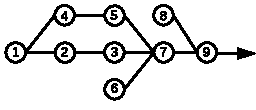
\includegraphics[width=0.8\textwidth]{ex-struct-process-1}}

\vspace{15pt}

Dove ogni {\it nodo numerato} rappresenta una {\it fase}. Ogni fase (nodo) ha zero o più fasi
che la {\it precedono} e zero o più fasi che la {\it seguono}. Le uniche regole da imporre
sono: deve esserci {\it una ed una sola} fase ($F_{9}$) che non ha alcuna fase successiva (un
solo {\it exit-node}), altrimenti si verrebbe a produrre più di un piatto (che è assurdo); non
devono esserci {\it cicli}, altrimenti la produzione del piatto non terminerebbe mai (altrettanto assurdo).

Con una struttura del genere è possibile ad esempio imporre che per iniziare una fase,
tutte le fasi precedenti ad essa devono essere portate a termine. Ad esempio nella struttura precedente:
$F_{5}$ può essere iniziata solo dopo che $F_{4}$ (e di conseguenza anche $F_{1}$) è stata completata.
$F_{7}$ può essere iniziata solo dopo che $F_{3}$ (e di conseguenza anche $F_{2}$ e $F_{1}$),
$F_{5}$ (e di conseguenza anche $F_{4}$) e $F_{6}$ sono state completate.

Possiamo inoltre {\it parallelizzare} la produzione del piatto. Ad esempio $F_{4}$ e $F_{5}$ possono essere
svolte da un cuoco mentre un altro cuoco sta svolgendo $F_{2}$ e $F_{3}$ (l'importante è che
$F_{1}$ sia stata portata a termine prima di iniziare $F_{2}$ e $F_{4}$). Nel mentre un altro
cuoco ancora può svolgere $F_{6}$ (in questo caso $F_{6}$ può iniziare anche prima di $F_{1}$)
e un altro ancora può svolgere $F_{8}$.

Per poter realizzare una struttura come questa in un database relazionale, sarà necessario
introdurre una {\it relazione ricorsiva}: l'entità che rappresenterà una fase dovrà essere
messa in una {\it relazione molti-a-molti} con se stessa. Infatti ogni fase deve essere
messa in relazione con le sue fasi precedenti (nell'immagine precedente: ogni collegamento
tra due fasi è una relazione).
La relazione ({\tt Precedente}) che permette la realizzazione di tale struttura è mostrata
nel {\it diagramma entità-relazione}~\vpageref{diagram.1}.
\subsection{Variazioni}\label{subsec:variations}
Con la struttura mostrata nel paragrafo \vref{sec:structuredprocess} è possibile anche
gestire le {\it variazioni}.

Le variazioni devono poter: aggiungere nuove fasi; rimuovere fasi.

Prendiamo ad esempio la seguente struttura che rappresenta il procedimento di una
pizza al prosciutto:

\vspace{5pt}\centerline{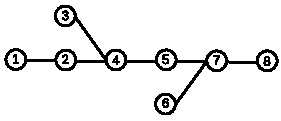
\includegraphics[width=0.8\textwidth]{ex-struct-process-2}}

\vspace{15pt}

Dove:
\begin{enumerate}[label=$F_{\arabic*}$:]
    \item fase di stesura della pasta;
    \item fase di aggiunta della pasta al piatto;
    \item fase di produzione del sugo di pomodoro;
    \item fase di aggiunta del pomodoro lavorato (sugo);
    \item fase di aggiunta della mozzarella;
    \item fase di taglio del prosciutto in fette;
    \item fase di aggiunta del prosciutto lavorato (fette di prosciutto);
    \item fase di cottura.
\end{enumerate}
\begingroup\itshape\fontsize{10pt}{10pt}\selectfont
    Si noti che con tale struttura ci sono più modi per rappresentare lo stesso procedimento
    di preparazione di un piatto: ad esempio si potrebbe scambiare $F_{1}$ con $F_{2}$ senza
    cambiare il \textnormal{senso} del procedimento; oppure si potrebbe spostare la fase $F_{7}$ a
    prima della fase $F_{6}$ e inserire una nuova fase al posto vuoto lasciato da $F_{7}$ che
    indica di mettere insieme i due \textnormal{semilavorati} (la pizza col pomodoro e la mozzarella
    e le fette di prosciutto).
\endgroup
\vspace{10pt}

Facciamo l'ipotesi che il cliente voglia come variazione la rimozione del pomodoro
(pizza bianca). In tal caso devono essere rimosse due fasi (anche se la variazione è
una sola!): $F_{3}$ e $F_{4}$. Se invece quello precedente fosse stato il procedimento
di una pizza margherita e il cliente avesse indicato come variazione l'aggiunta del
prosciutto, si sarebbero dovute aggiungere due fasi: $F_{6}$ e $F_{7}$.

Questo dimostra che è necessario che ogni variazione possa effettuare anche più di un'operazione
elementare (aggiunta o rimozione) sul procedimento strutturato.

L'entità {\tt ModificaFase} (con le sue entità figlie) è stata aggiunta al {\it diagramma
entità-relazione} (disponibile \vpageref{diagram.1}) allo scopo di permettere
ad ogni variazione di {\it modificare} anche più fasi: ogni variazione ha più
{\tt ModificaFase} e ogni {\tt ModificaFase} rappresenta la modifica (aggiunta, eliminazione, sostituzione)
di una e una sola fase (la sostituzione coinvolge però due fasi: quella da togliere e quella da aggiungere).

Le fasi che fanno parte di variazioni (come le fasi $F_{6}$ e $F_{7}$ nel caso del procedimento
della pizza margherita) non vengono confuse dal database con le fasi della ricetta {\it normale}:
infatti le fasi che fanno parte di variazioni si troveranno come {\it chiavi esterne}
all'interno dell'entità {\tt AggiuntaFase} (o {\tt SostituzioneFase}) per mezzo della relazione
{\tt Nuova}, e quindi il database saprà distinguerle da quelle della ricetta normale
(vedere il diagramma \vpageref{diagram.1}).

%\subsection{Ricetta originale e ricetta variata}
Dal procedimento strutturato deve essere possibile estrarre sia il procedimento della
ricetta originale (senza variazioni) sia il procedimento con una o più variazioni applicate.

Per vedere che ciò è possibile con il procedimento strutturato illustrato nel
paragrafo~\vref{sec:structuredprocess} è sufficiente notare che \ldots


\section{Rappresentazione concettuale}
\subsection{Entità}
Dalle specifiche di progetto e dal glossario dei termini prodotto nel
paragrafo~\vref{sec:termsglossary} del capitolo precedente, si individuano facilmente
le seguenti entità:
\begin{multicols}{3}
\begin{itemize}
    \item\tt Sede
    \item\tt Magazzino
    \item\tt Confezione
    \item\tt Ingrediente
    \item\tt Macchinario
    \item\tt Attrezzatura
    \item\tt Menu
    \item\tt Ricetta
    \item\tt Fase
    \item\tt Piatto
    \item\tt Variazione
    \item\tt ModificaFase
    \item\tt Comanda
    \item\tt Tavolo
    \item\tt Sala
    \item\tt Consegna
    \item\tt Pony
    \item\tt Prenotazione
\end{itemize}
\begin{itemize}
    \item\tt Account
    \item\tt Proposta
    \item\tt Suggerimento
    \item\tt Gradimento
    \item\tt Recensione
    \item\tt Valutazione
    \item\tt Questionario
    \item\tt Domanda
    \item\tt Risposta
    \item\tt QuestionarioSvolto
\end{itemize}
\end{multicols}
Queste entità sono state individuate procedendo con una strategia {\bf inside-out}
partendo da {\tt Sede} per l'area gestione e da {\tt Account} per l'area clienti. Come
si può infatti notare dalla lista dei collegamenti nel glossario dei termini, queste
entità sono fondamentali e contengono un alto numero di collegamenti: risulta quindi
facile muoversi {\it a macchia d'olio} partendo da queste.
Le entità della lista precedente sono poste nell'esatto ordine in cui sono state
aggiunte al diagramma durante la fase di progettazione concettuale.

\subsection{Generalizzazioni}
\begin{itemize}
\item Le due entità {\tt Attrezzatura} e {\tt Macchinario} sono entrambi
    strumenti da cucina. Condividono molte caratteristiche e per tal motivo è
    utile introdurre un'entità padre: {\tt Strumento}. La generalizzazione è
    {\it totale}, in quanto in cucina si possono avere solo attrezzature o
    macchinari, ed {\it esclusiva}.
\item Ogni {\tt Menu} che è stato sostituito da uno nuovo deve essere comunque
    mantenuto nel database. Per tale motivo è utile aggiungere l'entità
    {\tt MenuPassato} che rappresenta un menu non più in uso. In questo modo
    {\tt MenuPassato} è un sottoinsieme di {\tt Menu} e quindi è una generalizzazione
    {\it parziale}.
\item La {\tt Fase} può essere di due tipi: {\tt FaseIngrediente}, ossia di aggiunta
    di ingrediente, oppure {\tt FaseManovra}, ossia di lavorazione (con o senza strumento).
    La generalizzazione è {\it totale}. In teoria si potrebbe trattare come generalizzazione
    {\it sovrapposta}, ossia che una fase possa contenere sia l'aggiunta di un ingrediente
    sia una lavorazione (ad esempio: {\it affetta il prosciutto e aggiungilo al piatto}).
    Preferiamo però rendere le fasi quanto più elementari possibili. L'esempio precedente
    si può vedere anche come diviso in due fasi: {\it affetta il prosciutto}; {\it aggiungi il
    prosciutto}.
\item {\tt ModificaFase} può essere di due tipi: {\tt AggiuntaFase} oppure {\tt EliminazioneFase}.
    La generalizzazione è {\it totale} e {\it sovrapposta} (la sostituzione di una fase con
    un altra, infatti, altro non è che l'eliminazione di una fase e l'aggiunta di un'altra
    fase). Introduciamo quindi, per rendere {\it esclusiva} la generalizzazione, un'ulteriore
    entità: {\tt SostituzioneFase}.
\item La {\tt Comanda} può essere di due tipi: {\tt ComandaTavolo} oppure
    {\tt ComandaTakeAway}. La generalizzazione è {\it totale} ed
    {\it esclusiva}.
\item La {\tt Prenotazione} può essere di due tipi: una {\tt PrenotazioneOnline} (dal sito)
    oppure una {\tt PrenotazioneTelefonica}. La generalizzazione è {\it totale}
    ed {\it esclusiva}. Una {\tt PrenotazioneOnline} a sua volta può essere
    una semplice {\tt PrenotazioneOnline} oppure un {\tt Allestimento} (entità già individuata).
    In questo caso la generalizzazione è {\it parziale} e {\tt Allestimento}
    è un sottoinsieme di {\tt PrenotazioneOnline}.
\item {\it Variazione} e {\it Suggerimento} sono due entità molto simili tra loro: entrambe
    modificano una o più fasi del procedimento strutturato di una certa ricetta. Può quindi
    essere comodo generalizzarle in un'unica entità: rinominiamo quindi l'entità {\tt Variazione}
    in {\tt VariazionePiatto} così da poter utilizzare il nome {\tt Variazione} per l'entità
    padre di {\tt VariazionePiatto} e {\tt Suggerimento}. La generalizzazione è {\it totale}
    ed {\it esclusiva}.
\item Un {\tt Gradimento} può riferirsi a un {\tt Suggerimento} o a una {\tt Proposta}.
    Risulta quindi comodo aggiungere le entità {\tt GradimentoSuggerimento} e
    {\tt GradimentoProposta} come figlie. La generalizzazione è {\it totale} ed
    {\it esclusiva}.
\end{itemize}

Devono essere quindi aggiunte le seguenti entità:
\begin{multicols}{2}
\begin{itemize}
    \item\tt Strumento
    \item\tt MenuPassato
    \item\tt FaseIngrediente
    \item\tt FaseVariazione
    \item\tt AggiuntaFase
    \item\tt EliminazioneFase
    \item\tt SostituzioneFase
    \item\tt ComandaTavolo
    \item\tt ComandaTakeAway
    \item\tt PrenotazioneOnline
    \item\tt PrenotazioneTelefonica
    \item\tt VariazionePiatto
    \item\tt GradimentoSuggerimento
    \item\tt GradimentoProposta
\end{itemize}
\end{multicols}

\subsection{Associazioni}
Nella seguente tabella sono elencate e descritte tutte le relazioni, inserite
nell'ordine in cui sono state individuate.
{\tabulinesep=3pt
\begin{longtabu} to \linewidth {|X[c,m]|X[c,m]|X[c,m]|>{\raggedright}X[2,m]|}
\hline\rowfont\bfseries
Relazione   & \specialcell{Entità A\\(Cardinalità)}
                            & \specialcell{Entità B\\(Cardinalità)}
                                            & \centering Descrizione
\\ \hline \hline \hline \hline \hline % ----------------------------------------
\endhead
Disponibilità
            & \specialcell{Sede\\(1,N)}
                            & \specialcell{Magazzino\\(1,1)}
                                            & Una sede possiede uno o più magazzini.
                                              Un magazzino appartiene a una e una
                                              sola sede.
    \\ \hline % ----------------------------------------------------------------
Stoccaggio  & \specialcell{Magazzino\\(0,N)}
                            & \specialcell{Confezione\\(0,1)}
                                            & Le confezioni sono mantenute
                                              all'interno dei magazzini. Una confezione,
                                              rispetto a magazzino, può anche essere in ordine
                                              (e quindi non in stoccaggio).
    \\ \hline % ----------------------------------------------------------------
InOrdine    & \specialcell{Magazzino\\(0,N)}
                            & \specialcell{Confezione\\(0,1)}
                                            & Se una confezione non è in stoccaggio
                                              allora è in ordine. In questo caso
                                              non dovrà avere alcuni attributi (Collocazione,
                                              Aspetto, ecc.)
    \\ \hline % ----------------------------------------------------------------
Contenuto   & \specialcell{Confezione\\(1,1)}
                            & \specialcell{Ingrediente\\(0,N)}
                                            & Una confezione contiene uno e un solo
                                              tipo di ingrediente. Un certo ingrediente
                                              può essere contenuto in più confezioni (anche
                                              zero nel caso un ingrediente sia stato
                                              esaurito).
    \\ \hline % ----------------------------------------------------------------
Cucina      & \specialcell{Sede\\(0,N)}
                            & \specialcell{Strumento\\(1,N)}
                                            & La cucina mette in relazione gli strumenti
                                              con la sede alla quale appartengono.
                                              Dovrà riportare anche la quantità di strumenti
                                              di un certo tipo appartenenti alla sede.
    \\ \hline % ----------------------------------------------------------------
                                                                                                    %TODO: CONTINUARE TABELLA
\end{longtabu} }


%\section{Dizionario dei dati}

\section{Diagramma entità-relazione}\label{sec:conceptdiagram}
Il {\it diagramma concettuale} finale è mostrato \vpageref{diagram.1}.

Si noti che si è deciso di aggiungere una {\it ridondanza} nell'entità {\tt Comanda}:
l'attributo {\tt Stato} della comanda può infatti essere determinato dallo stato di
tutti i piatti ordinati nella comanda. Decidiamo però di mantenere tale ridondanza:
il motivo di questa decisione sarà discusso nel \vref{ch:redundancies}.

La spiegazione di come sono stati realizzati il {\it procedimento strutturato} e le {\it variazioni}
(e quindi anche i {\it suggerimenti}) è disponibile nel paragrafo \vref{sec:structuredprocess}.
\clearpage
\newgeometry{margin=2cm}
\thispagestyle{plain}
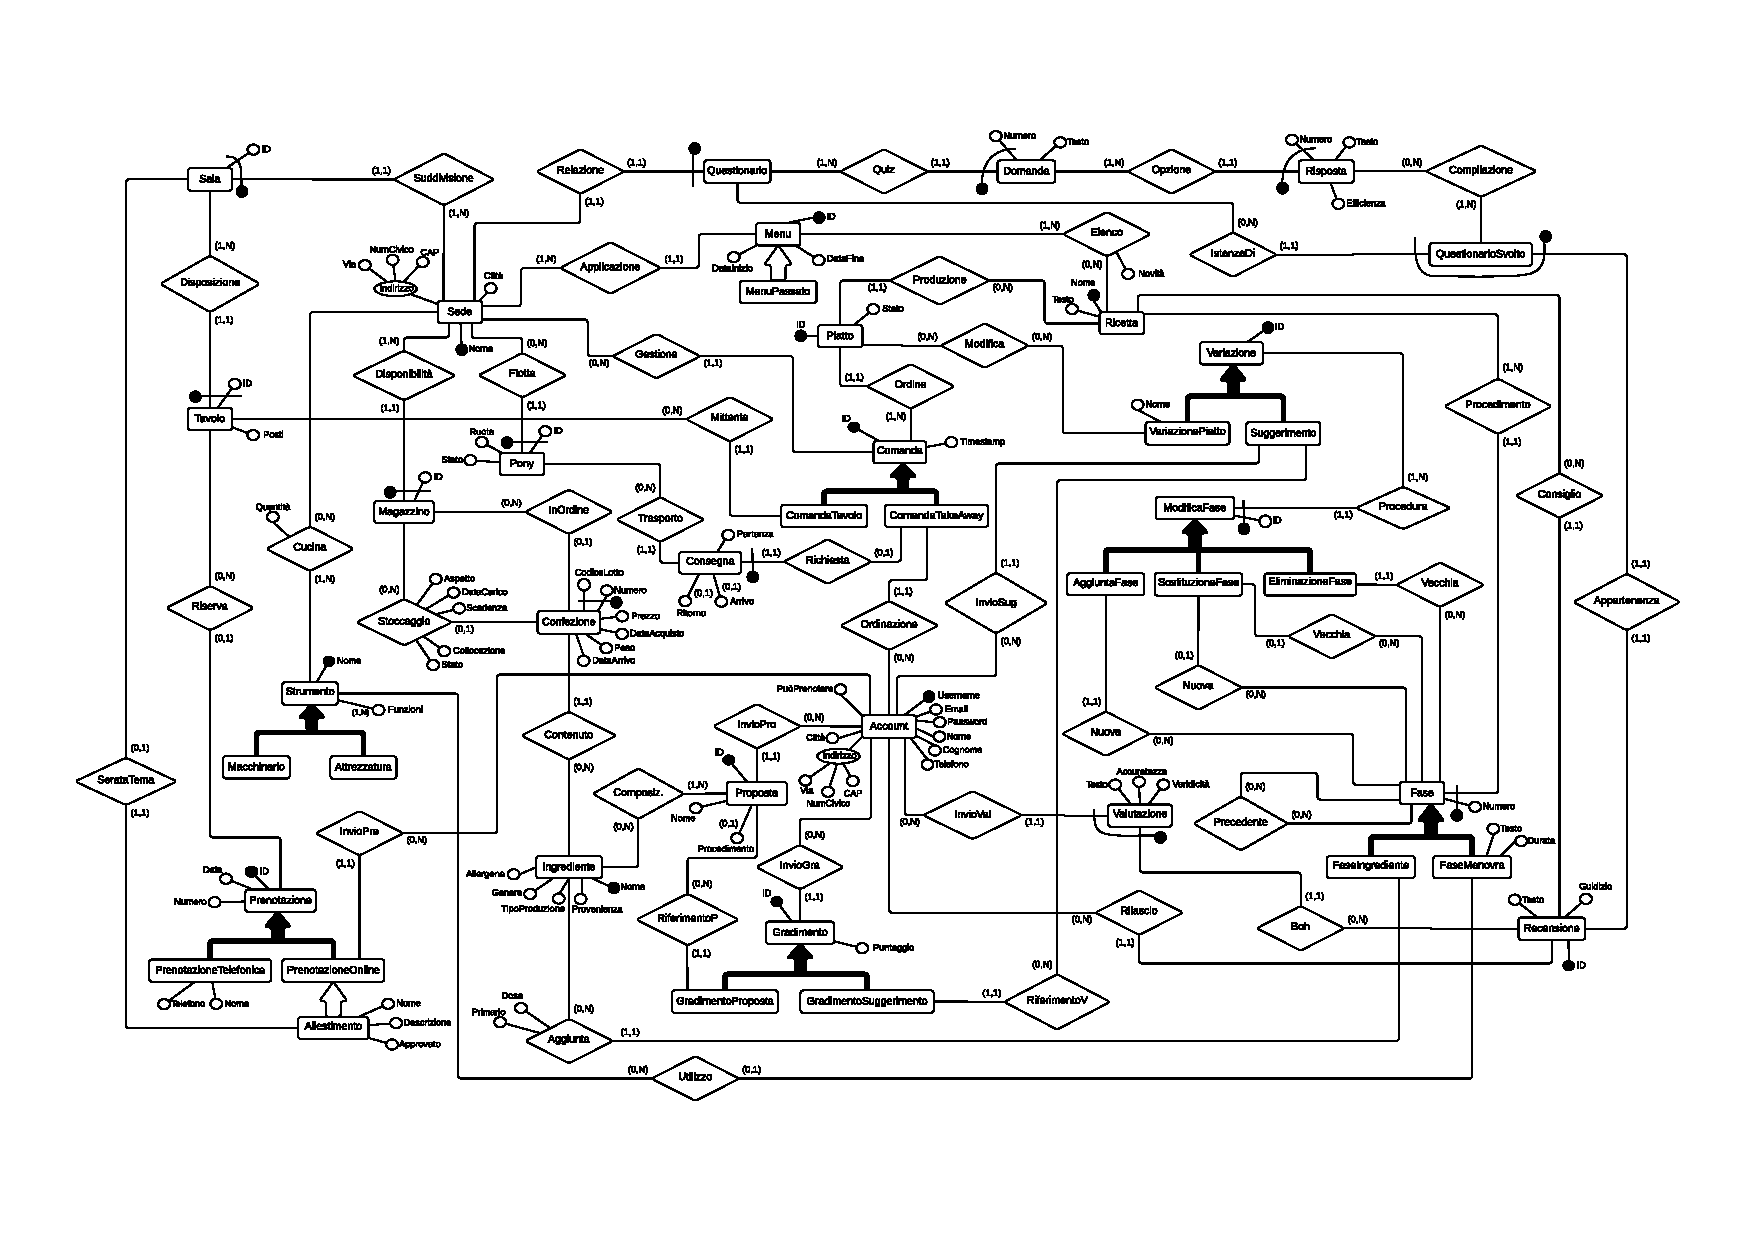
\includepdf[pages={1},landscape=true,pagecommand={\refstepcounter{includepdfpage}\label{diagram.\theincludepdfpage}}]{./images/diagrams.pdf}
\restoregeometry

        % Progettazione concettuale
\chapter{Ristrutturazione del diagramma E-R}
In questo Capitolo viene presentato il risultato della fase di {\it ristrutturazione del diagramma entità-relazione}. Il
paragrafo~\vref{sec:generalizations} descrive come sono state eliminate le {\it generalizzazioni}. Il
paragrafo~\vref{sec:multivalue} descrive come sono stati eliminati gli {\it attributi multivalore}. Il
paragrafo~\vref{sec:mergers} elenca gli altri accorpamenti effettuali per semplificare il diagramma. Infine,
il paragrafo~\vref{sec:restructureddiagram} riporta il {\it diagramma ristrutturato} finale.
\section{Eliminazione delle generalizzazioni}\label{sec:generalizations}
Di seguito viene mostrato come le generalizzazioni sono state eliminate per produrre
il {\it diagramma E-R ristrutturato}.

Nella totalità dei casi le generalizzazioni sono state eliminate {\bf accorpando
le entità figlie sull'entità padre}.

\vspace{15pt}

Nel caso della generalizzazione che coinvolge le entità {\tt Strumento}, {\tt Macchinario}
e {\tt Attrezzatura}, risulta comodo l'accorpamento sul padre in quanto {\tt Macchinario}
e {\tt Attrezzatura} non hanno attributi che il padre non possiede e non hanno
associazioni con altre entità.

\vspace{5pt}\centerline{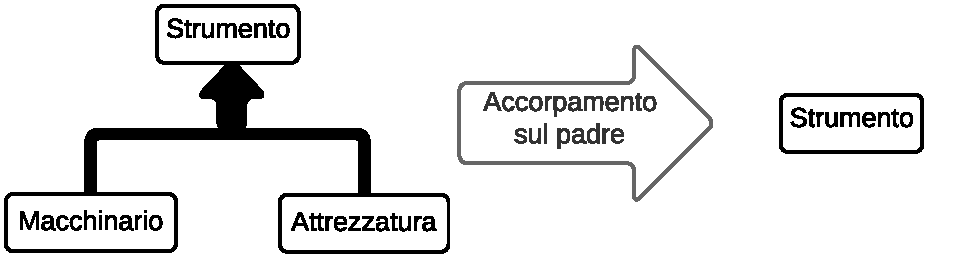
\includegraphics[width=\textwidth]{gen-strumento}}

\vspace{15pt}

Nel caso della generalizzazione che coinvolge le entità {\tt Menu} e  {\tt MenuPassato},
l'accorpamento sul padre non porta all'aggiunta di alcun attributo opzionale (l'attributo
{\tt DataFine} è inserito al momento dell'inserimento del menu nel database per BR\ldots).

\vspace{5pt}\centerline{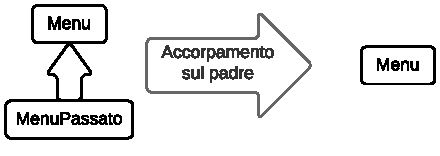
\includegraphics[width=0.8\textwidth]{gen-menu}}

\vspace{15pt}

Nel caso della generalizzazione che coinvolge le entità {\tt Fase}, {\tt FaseIngrediente}
e {\tt FaseManovra}, l'accorpamento sul padre porta all'introduzione di diversi attributi
opzionali: {\tt Durata}, {\tt Testo} ma anche {\tt Dose} e {\tt Primario} in quanto l'associazione
{\tt Aggiunta} diventa opzionale. Non è necessario inserire qui un attributo {\tt Tipo} per
riconoscere il tipo di fase in quanto può essere facilmente dedotto dalla presenza o meno
dell'associazione {\tt Aggiunta}.

\vspace{5pt}\centerline{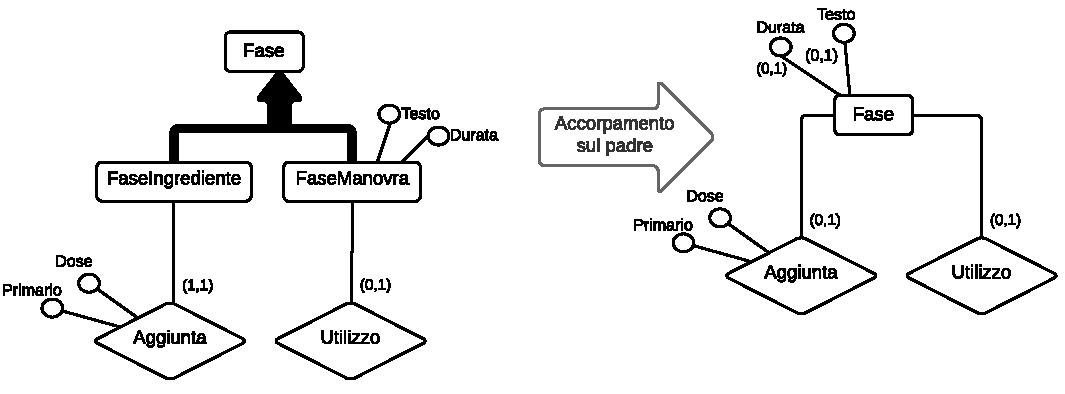
\includegraphics[width=\textwidth]{gen-fase}}

\vspace{15pt}

Nel caso della generalizzazione che coinvolge le entità {\tt Variazione}, {\tt VariazionePiatto}
e {\tt Suggerimento}, l'accorpamento sul padre porta all'aggiunta dell'attributo opzionale
{\tt Nome}. L'associazione {\tt InvioSug} diventa opzionale (e la rinominiamo in {\tt Suggerimento}).
Non è necessario inserire qui un attributo {\tt Tipo} per riconoscere il tipo di variazione
in quanto può essere facilmente dedotto dalla presenza o meno dell'associazione {\tt Suggerimento} (\hbox{ex-\texttt{InvioSug}}).

\vspace{5pt}\centerline{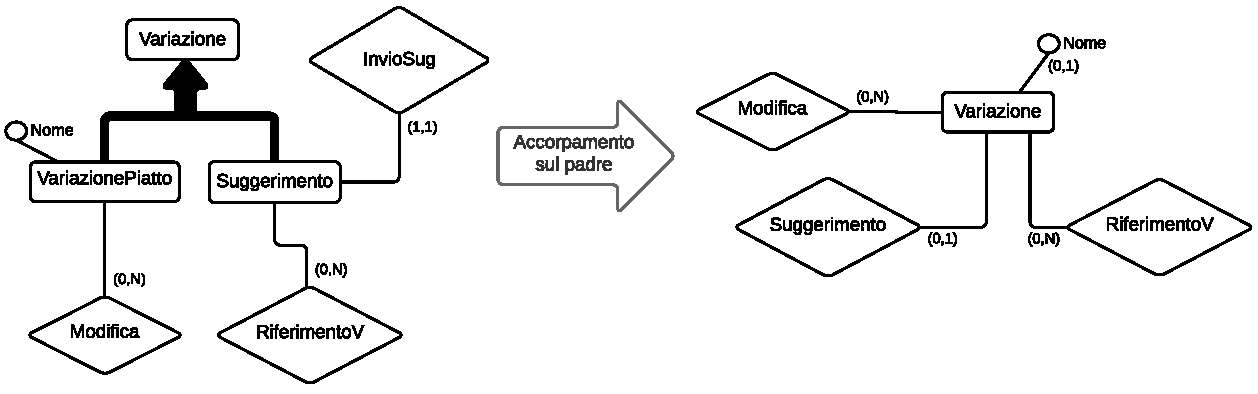
\includegraphics[width=\textwidth]{gen-variazione}}

\vspace{15pt}

Nel caso della generalizzazione che coinvolge le entità {\tt ModificaFase}, {\tt AggiuntaFase},
{\tt EliminazioneFase} e {\tt SostituzioneFase}, l'accorpamento sul padre porta all'eliminazione
di due associazioni (una {\tt Nuova} e una {\tt Vecchia}). Non è necessario introdurre qui un
attributo {\tt Tipo} per riconoscere il tipo di modifica di fase in quanto può essere facilmente
dedotto dalla presenza o meno delle associazioni {\tt Nuova} e {\tt Vecchia}: {\tt Nuova} = {\tt AggiuntaFase};
{\tt Vecchia} = {\tt EliminazioneFase}; {\tt Nuova} + {\tt Vecchia} = {\tt SostituzioneFase}.

\vspace{5pt}\centerline{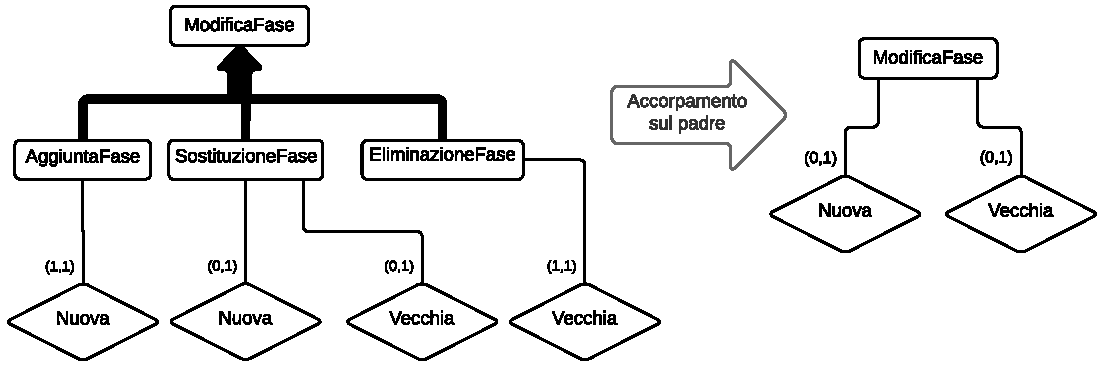
\includegraphics[width=\textwidth]{gen-modificafase}}

\vspace{15pt}

Nel caso della generalizzazione che coinvolge le entità {\tt Comanda}, {\tt ComandaTavolo}
e {\tt ComandaTakeAway}, l'accorpamento sul padre non porta all'aggiunta di attributi opzionali.
Ma le associazioni {\tt Mittente} e {\tt Ordinazione} diventano opzionali ({\tt Richiesta} è
già opzionale). Non è necessario inserire qui un attributo {\tt Tipo} per riconoscere
il tipo di comanda in quanto può essere facilmente dedotto dalla presenza o meno
dell'associazione {\tt Ordinazione}.

\vspace{5pt}\centerline{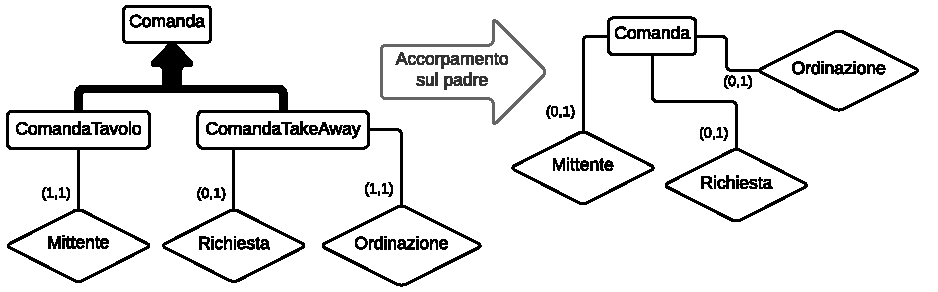
\includegraphics[width=\textwidth]{gen-comanda}}

\vspace{15pt}

Nel caso della generalizzazione che coinvolge le entità {\tt Gradimento}, {\tt GradimentoProposta}
e {\tt GradimentoSuggerimento}, l'accorpamento sul padre non porta all'aggiunta di attributi opzionali.
Ma le associazioni {\tt RiferimentoP} e {\tt RiferimentoS} diventano opzionali.
Non è necessario inserire qui un attributo {\tt Tipo} per riconoscere il tipo di
comanda in quanto può essere facilmente dedotto dall'associazione presente (se
{\tt RiferimentoP} o {\tt RiferimentoS}).

\vspace{5pt}\centerline{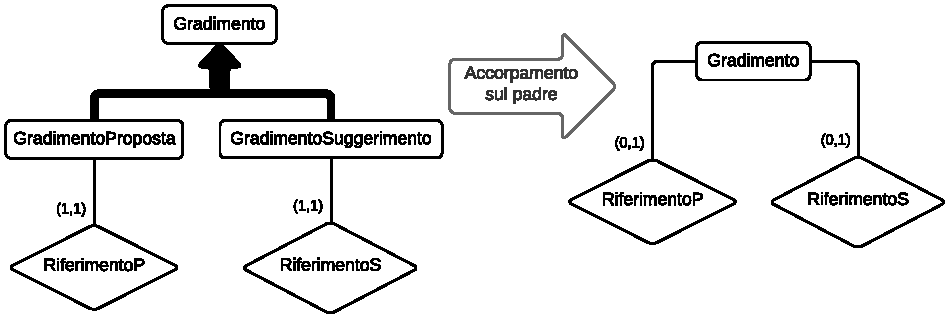
\includegraphics[width=\textwidth]{gen-gradimento}}

\vspace{15pt}

Nel caso delle due generalizzazioni che coinvolgono le entità {\tt Prenotazione},
{\tt PrenotazioneTelefonica}, {\tt PrenotazioneOnline} e {\tt Allestimento} si può
procedere con due accorpamenti sul padre: prima l'accorpamento di {\tt Allestimento}
su {\tt PrenotazioneOnline}; poi l'accorpamento di {\tt PrenotazioneTelefonica} e
{\tt PrenotazioneOnline} su {\tt Prenotazione}. Tutti gli attributi di {\tt PrenotazioneTelefonica}
e {\tt Allestimento} diventano opzionali, così anche le associazioni {\tt InvioPre}
e {\tt SerataTema}. Non è necessario inserire qui un attributo {\tt Tipo} per riconoscere
il tipo di prenotazione in quanto può essere facilmente dedotto dalla presenza o meno delle
associazioni {\tt InvioPre}, {\tt SerataTema} e {\tt Riserva}.

\vspace{5pt}\centerline{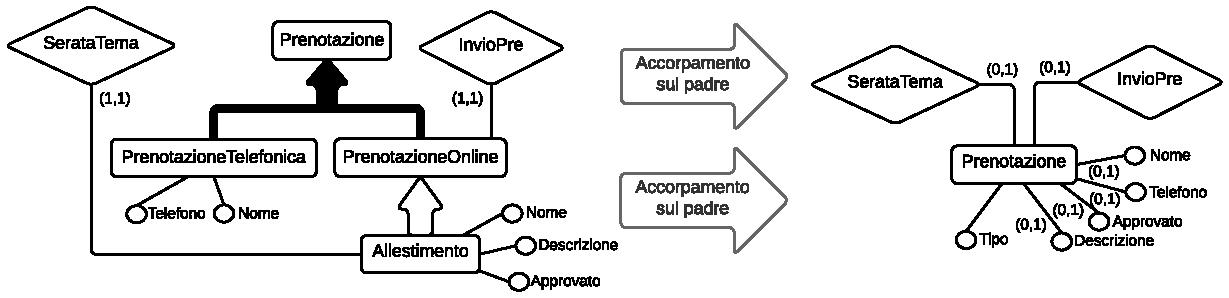
\includegraphics[width=\textwidth]{gen-prenotazione-allestimento}}

\section{Eliminazione di attributi multivalore}\label{sec:multivalue}
L'unico {\it attributo multivalore} presente nel diagramma è l'attributo {\tt Funzione} di {\tt Strumento}
con cardinalità {\tt (1,N)}. Questo attributo può essere facilmente eliminato aggiungendo
una nuova entità {\tt Funzione} legata a {\tt Strumento} tramite un'associazione {\it uno-a-molti}
come mostrato in figura:

\vspace{5pt}\centerline{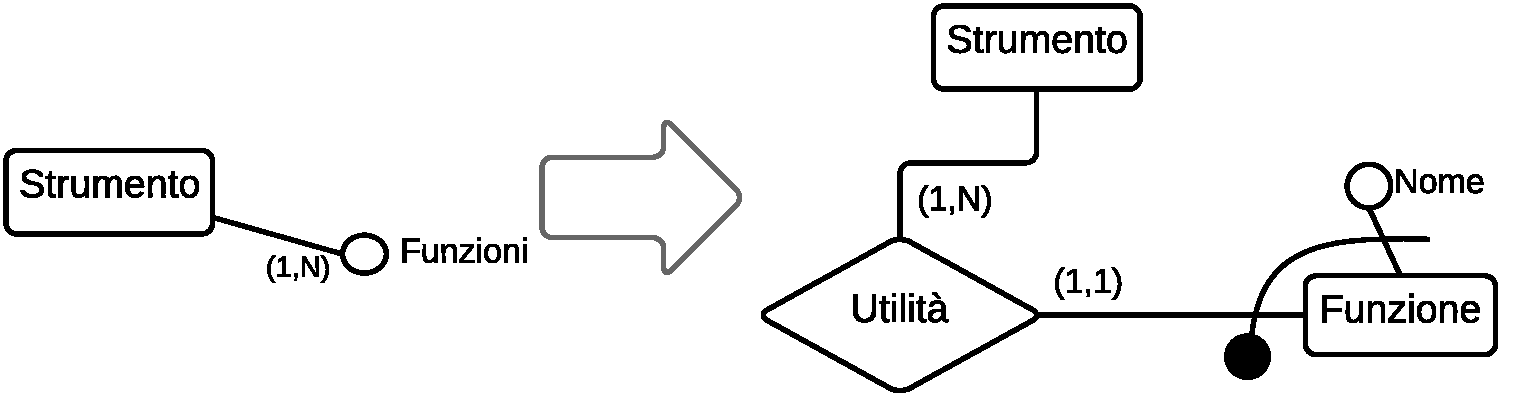
\includegraphics[width=\textwidth]{multi-funzione}}

% TODO: SPIEGARE PERCHÈ ABBIAMO DECISO DI FARE UNA RELAZIONE UNO-A-MOLTI INVECE CHE MOLTI-A-MOLTI

\section{Accorpamenti}\label{sec:mergers}
Possiamo effettuare altri accorpamenti al diagramma.\\

L'entità {\tt Questionario} e la relazione {\tt Relazione} che la collega all'entità {\tt Sede},
possono essere accorpate in un unica relazione {\tt Questionario} che lega {\tt Sede}
a {\tt Domanda} in quanto un questionario è identificato dalla sede alla quale appartiene
e non ha altri attributi.

Può essere fatto un ragionamento analogo al precedente anche per l'entità {\tt QuestionarioSvolto}
e la relazione {\tt Appartenenza} che la collega all'entità {\tt Recensione}. Viene
quindi rimossa anche la relazione {\tt IstanzaDi}.

%\section{Scelta degli identificatori principali}
Gli identificatori inseriti nel {\it diagramma concettuale} sarebbero già adeguati
per rappresentare le entità. Preferiamo però sostituire alcuni identificatori con
dei codici ({\tt ID}) per semplificare il diagramma e le relazioni con {\it chiavi
esterne identificative}.\\

Ad esempio si decide di utilizzare solo {\tt ID} come identificatore per l'entità
{\tt Piatto} in quanto:
\begin{inparaenum}[1)]
    \item dovrebbe in ogni caso mantenere l'attributo {\tt ID};
    \item nella relazione {\tt Modifica} dovremo inserire (se si decide di usare, oltre a {\tt ID},
        anche la chiave esterna con {\tt Comanda} e quella con {\tt Ricetta} come
        indetificatore principale) anche riferimenti {\tt Comanda} e {\tt Ricetta}.
\end{inparaenum}

Allo stesso modo si decide di utilizzare solo {\tt ID} come identificatore per
l'entità {\tt Recensione} in quanto:
\begin{inparaenum}[1)]
    \item dovrebbe in ogni caso mantenere l'attributo {\tt ID};
    \item nelle relazioni {\tt Valutazione} e {\tt QuestionarioSvolto} dovremo inserire
        (se si decide di usare, oltre a {\tt ID}, anche la chiave esterna con {\tt Account} come
        indetificatore principale) anche un riferimento a {\tt Account}.
\end{inparaenum}\\

Sono state fatte considerazioni analoghe anche per tutti gli altri identificatori
modificati nel {\it diagramma E-R ristrutturato}.

\section{Diagramma E-R ristrutturato}\label{sec:restructureddiagram}
Il {\it diagramma ristrutturato} finale è mostrato \vpageref{diagram.2}.
\clearpage
\newgeometry{margin=2cm}
\thispagestyle{plain}
\includepdf[pages={2},landscape=true,pagecommand={\refstepcounter{includepdfpage}\label{diagram.\theincludepdfpage}}]{./images/diagrams.pdf}
\restoregeometry

        % Ristrutturazione del diagramma E-R
\chapter{Progettazione logica}
\section{Traduzione del diagramma}\label{sec:translation}
In questo paragrafo discutiamo alcune scelte di traduzione effettuate nel passaggio
dal {\it diagramma E-R} allo {\it schema logico}.

%TODO: INSERIRE SPIEGAZIONI

\section{Schema logico}\label{sec:scheme}
Di seguito è mostrato lo {\it schema logico} risultante dalla fase di {\it progettazione logica}.

\vspace{10pt}
Si noti che le entità {\tt Comanda} e {\tt Consegna} potevano venir anche accorpate in un'unica entità. Abbiamo
però deciso di lasciarle separate così da evitare valori {\tt NULL} in più (nel caso di comanda da tavolo).

L'associazione {\tt Precedente} poteva anche essere tradotta con una tabella che riportasse
la fase {\it successiva} (invece della precedente). Non c'è alcuna differenza
tra l'una e l'altra rappresentazione --- decidiamo quindi di rappresentare la fase
{\it precedente} così da rimanere fedeli al nome dell'associazione.

Per tutte le {\it associazioni uno-a-molti con partecipazione opzionale}, ossia del tipo \hbox{\tt (0,1) --- (X,N)} (ad
esempio: {\tt Utilizzo}, {\tt Aggiunta}, {\tt Riserva}, {\tt Mittente}, ecc\ldots) si è sempre
deciso di {\bf non} creare una tabella aggiuntiva per l'associazione e di inserire invece
attributi opzionali. Questa scelta aumenta il numero di valori {\tt NULL} ma riduce il numero
di associazioni, e quindi anche il numero di accessi per le operazioni che coinvolgono tali
tabelle. Cerchiamo così di ottimizzare le prestazioni della base di dati.

Per il resto, la traduzione dal {\it diagramma entità-relazione ristrutturato} di pagina \pageref{diagram.2}
allo {\it schema logico} mostrato in questo paragrafo è del tutto ovvia e immediata. Non
sono quindi necessarie ulteriori spiegazioni.

\vspace{10pt}
Le {\it chiavi primarie} sono mostrate \underline{sottolineate} mentre gli {\it attributi opzionali}
sono rappresentati in \textit{corsivo}.

\begin{Verbatim}[commandchars=+\[\]]
SEDE(+underline[Nome], Città, CAP, Via, NumeroCivico)
MAGAZZINO(+underline[Sede], +underline[ID])
CONFEZIONE(+underline[CodiceLotto], +underline[Numero], Ingrediente, Peso, Prezzo, DataAcquisto,
    +textit[DataArrivo], +textit[DataCarico], Sede, Magazzino, +textit[Collocazione], Scadenza,
    +textit[Aspetto], Stato)
INGREDIENTE(+underline[Nome], Provenienza, TipoProduzione, Genere, Allergene)
CUCINA(+underline[Sede], +underline[Strumento], Quantità)
STRUMENTO(+underline[Nome])
FUNZIONE(+underline[Strumento], +underline[Nome])
MENU(+underline[ID], Sede, DataInizio, DataFine)
ELENCO(+underline[Menu], +underline[Ricetta], Novità)
RICETTA(+underline[Nome], Testo)
FASE(+underline[Ricetta], +underline[Numero], +textit[Ingrediente], +textit[Dose], +textit[Primario], +textit[Strumento], +textit[Testo],
    +textit[Durata])
SEQUENZAFASI(+underline[Ricetta], +underline[Fase], +underline[FasePrecedente])
PIATTO(+underline[ID], Comanda, Ricetta, Stato)
MODIFICA(+underline[Piatto], +underline[Variazione])
VARIAZIONE(+underline[ID], +textit[Nome], +textit[Account])
MODIFICAFASE(+underline[Variazione], +underline[ID], Ricetta, +textit[FaseVecchia], +textit[FaseNuova])
COMANDA(+underline[ID], Timestamp, Sede, +textit[Sala], +textit[Tavolo], +textit[Account])
TAVOLO(+underline[Sede], +underline[Sala], +underline[Numero], Posti)
SALA(+underline[Sede], +underline[Numero])
CONSEGNA(+underline[Comanda], Sede, Pony, Partenza, +textit[Arrivo], +textit[Ritorno])
PONY(+underline[Sede], +underline[ID], Ruote, Stato)
PRENOTAZIONE(+underline[ID], Sede, Data, Numero, +textit[Account], +textit[Nome], +textit[Telefono], Sala,
    +textit[Tavolo], +textit[Descrizione], +textit[Approvato])
ACCOUNT(+underline[Username], Email, Password, Nome, Cognome, Città, CAP, Via,
    NumeroCivico, Telefono, PuòPrenotare)
PROPOSTA(+underline[ID], Account, Nome, +textit[Procedimento])
COMPOSIZIONE(+underline[Proposta], +underline[Ingrediente])
GRADIMENTO(+underline[ID], Account, +textit[Proposta], +textit[Suggerimento], Punteggio)
RECENSIONE(+underline[ID], Account, Ricetta, Testo, Giudizio)
VALUTAZIONE(+underline[Account], +underline[Recensione], Veridicità, Accuratezza, Testo)
DOMANDA(+underline[Sede], +underline[Numero], Testo)
RISPOSTA(+underline[Sede], +underline[Domanda], +underline[Numero], Testo, Efficienza)
QUESTIONARIOSVOLTO(+underline[Recensione], +underline[Sede], +underline[Domanda], +underline[Risposta])
\end{Verbatim}

\section{Vincoli di integrità referenziale}
Di seguito riportiamo tutti i {\it vincoli di integrità referenziale} derivati dalla traduzione
delle associazioni nello schema logico.

{\tt R1(A) $\rightarrow$ R2(B)} indica che l'attributo {\tt A} della relazione {\tt R1}
è {\bf chiave esterna} dell'attributo {\tt B} della relazione {\tt R2} --- ossia che l'attributo
{\tt A} può assumere solo uno dei valori assunti dall'attributo {\tt B} (e il valore
{\tt NULL} se l'attributo è opzionale). Talvolta {\tt A} e {\tt B} possono essere
anche due {\it insiemi di attributi} con lo stesso numero di elementi, ognuno dei quali
separati da virgola.

Nella totalità dei casi, l'attributo (o l'insieme di attributi) {\tt B} è la
{\bf chiave primaria} della relazione {\tt R2}.

\begin{itemize}[parsep=0pt,listparindent=9\parindent]
    \item\tt MAGAZZINO(Sede)$\rightarrow$ SEDE(Nome)
    \item\tt CONFEZIONE(Magazzino, Sede) $\rightarrow$ MAGAZZINO(ID, Sede)
    \item\tt CONFEZIONE(Ingrediente) $\rightarrow$ INGREDIENTE(Nome)
    \item\tt CUCINA(Sede) $\rightarrow$ SEDE(Nome)
    \item\tt CUCINA(Strumento) $\rightarrow$ STRUMENTO(Nome)
    \item\tt FUNZIONE(Strumento) $\rightarrow$ STRUMENTO(Nome)
    \item\tt MENU(Sede) $\rightarrow$ SEDE(Nome)
    \item\tt ELENCO(Menu) $\rightarrow$ MENU(ID)
    \item\tt ELENCO(Ricetta) $\rightarrow$ RICETTA(Nome)
    \item\tt \ldots (FASE e VARIAZIONE) \ldots                                  % TODO: FASE E VARIAZIONE
    \item\tt PIATTO(Ricetta) $\rightarrow$ RICETTA(Nome)
    \item\tt PIATTO(Comanda) $\rightarrow$ COMANDA(ID)
    \item\tt COMANDA(Sede) $\rightarrow$ SEDE(Nome)
    \item\tt COMANDA(Tavolo, Sala, Sede) $\rightarrow$ TAVOLO(ID, Sala, Sede)
    \item\tt COMANDA(Account) $\rightarrow$ ACCOUNT(Username)
    \item\tt TAVOLO(Sala, Sede) $\rightarrow$ SALA(ID, Sede)
    \item\tt SALA(Sede) $\rightarrow$ SEDE(Nome)
    \item\tt CONSEGNA(Comanda) $\rightarrow$ COMANDA(ID)
    \item\tt CONSEGNA(Pony) $\rightarrow$ PONY(ID)
    \item\tt PONY(Sede) $\rightarrow$ SEDE(Nome)
    \item\tt PRENOTAZIONE(Account) $\rightarrow$ ACCOUNT(Username)
    \item\tt PRENOTAZIONE(Tavolo, Sala, Sede) $\rightarrow$ TAVOLO(ID, Sala, Sede)
    \item\tt PRENOTAZIONE(Sala, Sede) $\rightarrow$ SALA(ID, Sede)
    \item\tt PROPOSTA(Account) $\rightarrow$ ACCOUNT(Username)
    \item\tt COMPOSIZIONE(Proposta) $\rightarrow$ PROPOSTA(ID)
    \item\tt COMPOSIZIONE(Ingrediente) $\rightarrow$ INGREDIENTE(Nome)
    \item\tt SUGGERIMENTO(Account) $\rightarrow$ ACCOUNT(Username)
    \item\tt SUGGERIMENTO(Ricetta) $\rightarrow$ RICETTA(Nome)
    \item\tt GRADIMENTO(Account) $\rightarrow$ ACCOUNT(Username)
    \item\tt GRADIMENTO(Proposta) $\rightarrow$ PROPOSTA(ID)
    \item\tt GRADIMENTO(Suggerimento) $\rightarrow$ SUGGERIMENTO(ID)
    \item\tt RECENSIONE(Account) $\rightarrow$ ACCOUNT(Username)
    \item\tt RECENSIONE(Ricetta) $\rightarrow$ RICETTA(Nome)
    \item\tt VALUTAZIONE(Account) $\rightarrow$ ACCOUNT(Username)
    \item\tt VALUTAZIONE(Recensione) $\rightarrow$ RECENSIONE(ID)
    \item\tt DOMANDA(Sede) $\rightarrow$ SEDE(Nome)
    \item\tt RISPOSTA(Domanda, Sede) $\rightarrow$ DOMANDA(Numero, Sede)
    \item\tt QUESTIONARIOSVOLTO(Recensione) $\rightarrow$ RECENSIONE(ID)
    \item\tt QUESTIONARIOSVOLTO(Risposta, Domanda, Sede)
    
        $\rightarrow$ RISPOSTA(Numero, Domanda, Sede)
\end{itemize}

\section{Vincoli di integrità generici con MySQL}\label{sec:triggers}
Il seguente listato contiene i {\it trigger} necessari a effettuare tutti i controlli
di integrità generici per le tabelle del database.
Le descrizioni dei trigger sono inserite in blocchi di commento sopra al trigger
al quale si riferiscono.

\inputminted[%
              frame=leftline,           % bordo a sinistra
              linenos,                  % attiva numeri di linea
              stepnumber=5,             % solo multipli di 5 come numeri di linea
              tabsize=4,                % dimensione del tasto tab in spazi
              fontsize=\small]%         % dimensione del font (perché stia nella pagina bisogna assicurarsi che ogni riga di codice abbia al max 80 caratteri)
                              {mysql}{./sql/triggers.sql}

I {\it vincoli di integrità intrarelazionali semplici} ({\tt UNIQUE}, {\tt UNSIGNED}, {\tt CHECK}, ecc.)
sono riportati solo ~\vref{ch:sqlcode}.

        % Progettazione logica
\chapter{Normalizzazione}
In questo Capitolo viene presentato il risultato della fase di {\it normalizzazione}.

Nel paragrafo~\vref{sec:functionaldependencies} è presentata la lista di tutte le {\it dipendenze
funzionali non banali}. Nei paragrafi ad esso successivi viene riportata la normalizzazione
di tutte le relazioni che non rispettano la {\bf Forma Normale di Boyce-Codd (BCNF)}.
% Si può notare facilmente che le uniche due tabelle a presentare
%dipendenze funzionali non banali che violano la {\bf Forma Normale di Boyce-Codd (BCNF)}
%sono:
%\begin{itemize}
%\item {\tt Sede}: {\tt Città}, {\tt Via} $\rightarrow$ {\tt CAP}
%\item {\tt Account}: {\tt Città}, {\tt Via} $\rightarrow$ {\tt CAP}
%\end{itemize}
%Queste dipendenze funzionali {\it non} sono però normalizzabili (a meno di non avere una tabella
%che metta in relazione tutte le coppie ({\tt Città}, {\tt Via}) con il relativo {\tt CAP}). Si
%noti inoltre che, per quanto riguarda la relazione {\tt Sede}, non saranno mai presenti
%due sedi con la stessa coppia ({\tt Città}, {\tt Via}) --- è infatti assurdo che una catena
%di ristorazione possieda più di una sede nella stessa via --- e quindi la {\it decomposizione}
%di tale dipendenza funzionale non porterebbe a nessun vantaggio. Per quanto riguarda la
%relazione {\tt Account}, l'introduzione dell'attributo {\tt CAP} non è richiesto dalle
%specifiche e non è necessario in quanto il {\it Codice di Avviamento Postale} è utile solo
%nel caso in cui sia necessario spedire un bene utilizzando i {\it servizi postali italiani}: le
%uniche {\it spedizioni} effettuate dalla catena di ristorazione sono le {\it consegne a
%domicilio} effettuate dai {\it pony}, che non hanno bisogno del {\it CAP} --- volendo quindi
%normalizzare anche la tabella {\tt Account}, si potrebbe semplicemente eliminare l'attributo {\tt CAP}.

Vediamo ora tutte le {\it dipendenze funzionali non banali}.
\section{Dipendenze funzionali}\label{sec:functionaldependencies}

\section{Sede e Account}\label{sec:sedeaccount}
Le relazioni {\tt Sede} e {\tt Account} non rispettano la BCNF. A causare il problema
sono le seguenti dipendenze funzionali:
\begin{itemize}
\item {\tt Sede}: {\tt Città}, {\tt Via} $\rightarrow$ {\tt CAP}
\item {\tt Account}: {\tt Città}, {\tt Via} $\rightarrow$ {\tt CAP}
\end{itemize}
Queste dipendenze funzionali {\it non} sono però normalizzabili (a meno di non avere una tabella
che metta in relazione tutte le coppie ({\tt Città}, {\tt Via}) con il relativo {\tt CAP}). Si
noti inoltre che, per quanto riguarda la relazione {\tt Sede}, non saranno mai presenti
due sedi con la stessa coppia ({\tt Città}, {\tt Via}) --- è infatti assurdo che una catena
di ristorazione possieda più di una sede nella stessa via --- e quindi la {\it decomposizione}
di tale dipendenza funzionale non porterebbe a nessun vantaggio. Per quanto riguarda la
relazione {\tt Account}, l'introduzione dell'attributo {\tt CAP} non è richiesto dalle
specifiche e non è necessario in quanto il {\it Codice di Avviamento Postale} è utile solo
nel caso in cui sia necessario spedire un bene utilizzando i {\it servizi postali italiani}: le
uniche {\it spedizioni} effettuate dalla catena di ristorazione sono le {\it consegne a
domicilio} effettuate dai {\it pony}, che non hanno bisogno del {\it CAP} --- volendo quindi
normalizzare anche la tabella {\tt Account}, si potrebbe semplicemente eliminare
l'attributo {\tt CAP}.\footnote{In questo progetto l'attributo {\tt CAP} sarà comunque mantenuto sia per {\tt Sede} che per {\tt Account}.}

\section{Confezione}\label{sec:confezione}
La relazione {\tt Confezione} non rispetta la BCNF. Riportiamo di seguito tutte
le dipendenze funzionali non banali della relazione in questione:
\begin{funcdep}{Confezione}
    CodiceLotto $\to$ Ingrediente, Scadenza\\
    CodiceLotto, Numero $\to$ Peso, Prezzo, DataAcquisto, DataCarico,\\
        \indent\indent\indent\indent\indent DataArrivo, Sede, Magazzino, Collocazione,\\
        \indent\indent\indent\indent\indent Aspetto, Stato
\end{funcdep}

\noindent\texttt{CodiceLotto}, da sé, non è infatti {\it superchiave} della relazione {\tt Confezione}.
Per poter normalizzare tale relazione è necessario scomporla in due relazioni:

\begin{Verbatim}[commandchars=+\[\]]
CONFEZIONE(+underline[CodiceLotto], +underline[Numero], Peso, Prezzo, DataAcquisto, +textit[DataCarico],
    +textit[DataArrivo], Sede, Magazzino, +textit[Collocazione], +textit[Aspetto], +textit[Stato])
LOTTO(+underline[Codice], Ingrediente, Scadenza)
\end{Verbatim}
Dobbiamo anche aggiungere il {\it vincolo di integrità referenziale} tra {\tt CodiceLotto}
di {\tt Confezione} e {\tt Codice} di {\tt Lotto}.

\vspace{10pt}
\noindent Si vede immediatamente che, così facendo, la BCNF è rispettata.

\section{ModificaFase}\label{sec:modificafase}
La relazione {\tt ModificaFase} non rispetta la BCNF. Riportiamo di seguito tutte
le dipendenze funzionali non banali della relazione in questione:
\begin{funcdep}{ModificaFase}
    Variazione $\to$ Ricetta\\
    Variazione, ID $\to$ FaseVecchia, FaseNuova
\end{funcdep}
\noindent\texttt{Variazione}, da sé, non è infatti {\it superchiave} della relazione {\tt ModificaFase}.
Per poter normalizzare tale relazione è necessario spostare l'attributo {\tt Ricetta} nella
relazione {\tt Variazione}. Questo però ci impone anche di dover trovare un nuovo identificatore
per {\tt Fase} --- useremo quindi un campo {\tt ID} e toglieremo {\tt Numero} (superfluo in quanto l'ordine
delle fasi è dato dalla relazione {\tt SequenzaFasi}). Bisognerà quindi modificare le
relazioni coinvolte come segue:

\begin{Verbatim}[commandchars=+\[\]]
FASE(+underline[ID], Ricetta, +textit[Ingrediente], +textit[Dose], +textit[Primario], +textit[Strumento], +textit[Testo],
    +textit[Durata])
SEQUENZAFASI(+underline[Fase], +underline[FasePrecedente])
VARIAZIONE(+underline[ID], Ricetta, +textit[Nome], +textit[Account])
MODIFICAFASE(+underline[Variazione], +underline[ID], +textit[FaseVecchia], +textit[FaseNuova])
\end{Verbatim}
Anche i {\it vincoli di integrità referenziale} dovranno cambiare di conseguenza: dovrà
essere aggiunto il vincolo tra {\tt Ricetta} di {\tt Variazione} e {\tt Nome} di {\tt Ricetta}; dovranno
inoltre essere sistemati tutti i vincoli che si riferiscono alle tuple di {\tt Fase} in quanto
adesso vengono identificate dall'unico attributo {\tt ID}.

\vspace{10pt}
\noindent Si vede immediatamente che, così facendo, la BCNF è rispettata per tutte le relazioni modificate.

\section{QuestionarioSvolto}\label{sec:questionariosvolto}
La relazione {\tt QuestionarioSvolto} non rispetta la BCNF. Riportiamo di seguito tutte
le dipendenze funzionali non banali della relazione in questione:
\begin{funcdep}{QuestionarioSvolto}
    Recensione $\to$ Sede\\
    Recensione, Sede, Domanda $\to$ Risposta
\end{funcdep}
\noindent\texttt{Recensione}, da sé, non è infatti {\it superchiave} della relazione {\tt QuestionarioSvolto}. Per
poter normalizzare tale relazione è necessario spostare l'attributo {\tt Sede} nella
relazione {\tt Recensione}. Questo però ci impone anche di dover trovare un nuovo identificatore
per le relazioni {\tt Risposta} e {\tt Domanda} --- useremo quindi un campo {\tt ID} per {\tt Domanda} e
toglieremo {\tt Numero} (superfluo in quanto l'ordine delle domande può essere dato dalla sequenza
degli {\tt ID}). Inoltre possiamo (anche se non necessario per la normalizzazione)
togliere {\tt Risposta} dall'identificatore di {\tt QuestionarioSvolto} (è
possibile in quanto, per ogni recensione, l'utente può dare una sola risposta ad ogni
domanda --- come specificato dalla business rule \ref{br.surveyanswers}). Bisognerà
quindi modificare le relazioni coinvolte come segue:

\begin{Verbatim}[commandchars=+\[\]]
RECENSIONE(+underline[ID], Account, Sede, Ricetta, Testo, Giudizio)
DOMANDA(+underline[ID], Sede, Testo)
RISPOSTA(+underline[Domanda], +underline[Numero], Testo, Efficienza)
QUESTIONARIOSVOLTO(+underline[Recensione], +underline[Domanda], Risposta)
\end{Verbatim}
Anche i {\it vincoli di integrità referenziale} dovranno cambiare di conseguenza: dovrà
essere aggiunto il vincolo tra {\tt Sede} di {\tt Recensione} e {\tt Nome} di {\tt Sede}; dovranno
inoltre essere sistemati il vincolo tra {\tt QuestionarioSvolto} e {\tt Risposta} in quanto le tuple di quest'ultima
adesso vengono identificate dai soli attributi {\tt Domanda} e {\tt Numero}. Ovviamente deve essere
sistemato anche il vincolo tra {\tt Risposta} e {\tt Domanda} in quanto le tuple di quest'ultima adesso
vengono identificate dall'unico attributo {\tt ID}.

\vspace{10pt}
\noindent Si vede immediatamente che, così facendo, la BCNF è rispettata per tutte le relazioni modificate.

        % Normalizzazione
\chapter{Operazioni}
\section{Individuazione delle operazioni}
\section{Implementazione delle operazioni}
        % Operazioni
\chapter{Operazioni}\label{ch:operations}
In questo Capitolo sono presentate alcune {\it operazioni interessanti}. Successivamente, nel
paragrafo~\vref{sec:operationscode}, saranno presentate le {\it implementazioni MySQL} di tali operazioni.
\section{Implementazione delle operazioni}\label{sec:operationscode}
        % Analisi delle prestazioni
\chapter{Analisi delle prestazioni}
In questo Capitolo viene presentato il risultato della fase di {\it analisi delle prestazioni} di
alcune operazioni interessanti. Il paragrafo~\vref{sec:volumetable} riporta la tavola dei
volumi delle {\it tabelle} del database. Il paragrafo~\vref{sec:accesstables} riporta, per ogni
operazione individuata nel Capitolo~\vref{ch:operations}, la {\it tavola degli accessi}.
\section{Tavola dei volumi}\label{sec:volumetable}
La {\it tavola dei volumi} seguente contiene tre colonne: la prima riporta il nome della
{\it tabella} che si considera; la seconda contiene il {\it volume stimato} della tabella; la terza
{\it descrive} come è stata calcolata la stima.

Ogni qual volta che si riporta il nome di una tabella in una {\it espressione matematica} si deve
intendere il {\it volume della tabella}.

{\tabulinesep=3pt
\begin{longtabu} to \linewidth {|>{\large}X[c,m]|>{\Large}X[c,m]|>{\raggedright}X[3,m]|}
\hline\rowfont\bfseries
{\Large Tabella}& Volume        & \centering {\Large Commento}
\\ \hline \hline \hline \hline \hline % ----------------------------------------
\endhead
Sede            & \(25\)        & Ipotesi: la catena di ristorazione ha \(25\) sedi.
    \\ \hline % ----------------------------------------------------------------
Magazzino       & \(50\)        & Ogni sede ha in media 2 magazzini: \(2 \times Sede = 50\).
    \\ \hline % ----------------------------------------------------------------
Confezione      & \(20\,000\)   & Ogni magazzino ha in media 400 confezioni (alcune in ordine): \(400 \times Magazzino = 20\,000\).
    \\ \hline % ----------------------------------------------------------------
Ingrediente     & \(150\)       & Ipotesi: ci sono \(150\) ingredienti possibili.
    \\ \hline % ----------------------------------------------------------------
Lotto           & \(1\,500\)    & La catena di ristorazione possiede (nello stesso momento) \(10\)
                                  lotti per ogni ingrediente (eliminiamo i lotti per i quali
                                  non sono più presenti confezioni in alcun magazzino).
    \\ \hline % ----------------------------------------------------------------
Cucina          & \(750\)       & \(Strumento \times Sede = 750\).
    \\ \hline % ----------------------------------------------------------------
Strumento       & \(50\)        & Ipotesi: ci sono \(50\) strumenti possibili.
    \\ \hline % ----------------------------------------------------------------
Funzione        & \(150\)       & Ogni strumento ha in media 3 funzioni: \(3 \times Strumento = 150\).
    \\ \hline % ----------------------------------------------------------------
Menu            & \(500\)       & Ogni sede ha applicato (nel tempo) in media 20 menu: \(20 \times Sede = 500\). In
                                   realtà il numero di menu cresce anche di molto nel tempo (dipende dalla frequenza
                                   con cui una sede cambia menu e dal tempo trascorso), ma 500 può essere
                                   un'approssimazione adeguata.
    \\ \hline % ----------------------------------------------------------------
Elenco          & \(10\,000\)   & Ogni menu elenca in media 20 ricette: \(20 \times Menu = 10\,000\).
    \\ \hline % ----------------------------------------------------------------
Ricetta         & \(200\)       & Ipotesi: il ricettario della catena di ristorazione è formato da \(200\) ricette.
    \\ \hline % ----------------------------------------------------------------
Fase            & \(5\,000\)    & Ogni ricetta ha in media dalle 20 alle 25 fasi (quindi circa 22); inoltre
                                  in media \(\sfrac{2}{3}\) delle istanze di ModificaFase
                                  richiedono l'aggiunta di una nuova fase:
                                  \(\approx 22 \times Ricetta + \frac{2}{3} ModificaFase = 4\,900 \approx 5\,000\).
    \\ \hline % ----------------------------------------------------------------
SequenzaFasi    & \(7\,500\)    & Ogni fase ha in media una o due fasi che la precedono: \(1.5 \times Fase = 7\,500\).
    \\ \hline % ----------------------------------------------------------------
Piatto          & \specialcell{\(\infty\)\\\((\approx 500\,000)\)}
                                & Ogni comanda ordina in media 5 piatti: \(5 \times Comanda = 500\,000\). Si
                                  veda anche la nota a fine tavola (\(\infty\)).
    \\ \hline % ----------------------------------------------------------------
Modifica        & \specialcell{\(\infty\)\\\((\approx 25\,000)\)}
                                & In media un piatto su 25 applica una variazione (o
                                  più di una --- al massimo 3). Approssimiamo quindi a
                                  \(\sfrac{1}{20} = 0.05\):
                                  \(\approx 0.05 \times Piatto = 25\,000\). Si
                                  veda anche la nota a fine tavola (\(\infty\)).
    \\ \hline % ----------------------------------------------------------------
Variazione      & \(1\,000\)    & Ogni ricetta ha in media due variazioni possibili; inoltre
                                  si ipotizza che gli utenti della piattaforma web rilascino
                                  600 suggerimenti: \(2 \times Ricetta + 600 = 1\,000\).
    \\ \hline % ----------------------------------------------------------------
ModificaFase    & \(1\,500\)    & Ogni variazione in media richiede la modifica di una o due
                                  fasi: \(1.5 \times Variazione = 1\,500\).
    \\ \hline % ----------------------------------------------------------------
Comanda         & \specialcell{\(\infty\)\\\((\approx 100\,000)\)}
                                & Ipotesi: ogni giorno la metà dei tavoli di una sede sono occupati (considerando
                                  anche che la sede può fare più di un turno); ognuno di questi tavoli,
                                  in quel turno, invia una o due comande; inoltre si ipotizza che ogni
                                  giorno ogni sede riceva 5 comande take-away:
                                  \(\sfrac{Tavolo}{2} \times 1.5 \approx 550 + 5 \times Sede \approx 675/giorno\). Per
                                  il volume totale della tabella approssimiamo quindi ad un
                                  numero molto alto: \(\approx 100\,000\). Si
                                  veda anche la nota a fine tavola (\(\infty\)).
    \\ \hline % ----------------------------------------------------------------
Tavolo          & \(750\)       & Ogni sala ha in media 15 tavoli: \(15 \times Sala = 750\).
    \\ \hline % ----------------------------------------------------------------
Sala            & \(50\)        & Ogni sede ha in media 2 sale: \(2 \times Sede = 50\).
    \\ \hline % ----------------------------------------------------------------
Consegna        & \specialcell{\(\infty\)\\\((\approx 10\,000)\)}
                                & Ipotesi: ogni giorno ogni sede riceve 5 comande take-away: \(5 \times Sede = 125/giorno\). Per
                                  il volume totale della tabella approssimiamo quindi ad un
                                  numero alto: \(\approx 10\,000\). Si veda anche
                                  la nota a fine tavola (\(\infty\)).
    \\ \hline % ----------------------------------------------------------------
Pony            & \(100\)       & Ogni sede ha in media 4 pony: \(4 \times Sede = 100\).
    \\ \hline % ----------------------------------------------------------------
Prenotazione    & \specialcell{\(\infty\)\\\((\approx 50\,000)\)}
                                & Ipotesi: ogni giorno ogni sede riceve 15 prenotazioni: \(15 \times Sede = 375/giorno\). Per
                                  il volume totale della tabella approssimiamo quindi ad un
                                  numero alto: \(\approx 50\,000\). Si veda anche
                                  la nota a fine tavola (\(\infty\)).
    \\ \hline % ----------------------------------------------------------------
Account         & \(10\,000\)   & Ipotesi: nel tempo si registrano circa \(10\,000\) utenti.
    \\ \hline % ----------------------------------------------------------------
Proposta        & \(1\,000\)    & In media {\it meno} di un utente su 10 rilascerà una proposta
                                  sulla piattaforma web, però qualcuno di questi utenti ne rilascerà
                                  più di una. Approssimiamo quindi a \(\sfrac{1}{10} = 0.1\):
                                  \(\approx 0.1 \times Account = 1\,000\).
    \\ \hline % ----------------------------------------------------------------
Composizione    & \(7\,000\)     & Una ricetta (anche quelle proposte) in media è composta da
                                  7 ingredienti: \(7 \times Proposta = 7\,000\).
    \\ \hline % ----------------------------------------------------------------
Gradimento      & \(4\,800\)    & Ogni proposta ha in media 3 gradimenti; ogni suggerimento
                                  ha in media 3 gradimenti: \(3 \times Proposta + 3 \times Suggerimento = 4\,800\).
    \\ \hline % ----------------------------------------------------------------
Recensione      & \(2\,000\)    & In media solo un utente su 10 si preoccuperà di
                                  rilasciare recensioni sul sito; ognuno di questi
                                  rilascerà in media 2 recensioni: \(2 \times 0.1 \times Account = 2\,000\).
    \\ \hline % ----------------------------------------------------------------
Valutazione     & \(4\,000\)    & Ogni recensione ha in media 2 valutazioni: \(2 \times Recensione = 4\,000\).
    \\ \hline % ----------------------------------------------------------------
Domanda         & \(125\)       & Ogni sede ha un questionario (insieme di domande); ognuno
                                  di questi questionari è composto in media da 5 domande:
                                  \(5 \times Sede = 125\).
    \\ \hline % ----------------------------------------------------------------
Risposta        & \(375\)       & Ogni domanda ha in media 3 risposte possibili: \(3 \times Domanda = 375\).
    \\ \hline % ----------------------------------------------------------------
\specialcell{Questionario--\\Svolto}
                & \(1\,000\)    & La tabella {\tt QuestionarioSvolto} mette in relazione
                                  {\tt Recensione} e {\tt Risposta} associando ad ogni
                                  recensione le varie risposte date al questionario. Ogni
                                  questionario è composto in media da 5 domande: \(Recensione \times 5 = 1\,000\).
    \\ \hline % ----------------------------------------------------------------
Clienti\_Log    & \(1\,500\)
                                & Se la catena di ristorazione è aperta da 5
                                  anni: \(\approx Sede \times 5 \times 12 = 1\,500\).
    \\ \hline % ----------------------------------------------------------------
Scarichi\_Log   & \(7\,500\)    & \(Ingrediente \times Magazzino = 7\,500\).
    \\ \hline % ----------------------------------------------------------------
\specialcell{MV\_Ordini--\\Ricetta}
                & \(5\,000\)    & \(Sede \times Ricetta = 5\,000\).
    \\ \hline % ----------------------------------------------------------------
\specialcell{MV\_Menu--\\Corrente}
                & \(500\)       & Ogni menu elenca in media 20 ricette: \(Sede \times Elenco = 500\).
    \\ \hline % ----------------------------------------------------------------
\end{longtabu} }

\noindent{\large\bf NOTA (\(\infty\)):}

Per alcune tabelle ({\tt Comanda}, {\tt Piatto}, ecc\ldots) al posto del volume è stato
inserito il simbolo di infinito (\(\infty\)) e, tra parentesi, un'approssimazione del volume. Per
queste tabelle non è possibile fare una stima che si possa ritenere {\it precisa} del volume in
quanto dipendente da fattori molto aleatori (come il tempo).

Ad esempio il numero di comande (e quindi anche dei piatti ordinati) aumenta notevolmente
via via che il tempo passa: dopo un intero anno il volume della tabella {\tt Comanda} può essere
anche di {\it centinaia di migliaia di record}; dopo 5 anni il volume della tabella {\tt Piatto} può
essere anche di {\it qualche milione di record}. Ovviamente non ha senso mantenere per sempre (o
molto a lungo) le informazioni sulle comande e sui piatti ordinati e l'amministratore
dovrebbe occuparsi di ripulire il database da informazioni non più utili\footnote{La base di %
dati di questo progetto non contiene funzionalità per la pulizia di informazioni %
ritenute superflue: l'eventuale pulizia del database, se desiderata, è lasciata %
all'intervento manuale dell'amministratore.}. Stimiamo però comunque
valori molto alti per il volume di queste tabelle, così da tenere in considerazione il
caso in cui l'amministratore non provveda molto frequentemente alla pulizia del database. Il
valore così stimato è inserito, nella tavola, tra parentesi tonde sotto il simbolo \(\infty\). Questo
valore sarà quello utilizzato per tutte le stime di qui in poi (ad esempio, nelle
{\it tavole degli accessi} per le operazioni).

\section{Tavole degli accessi}\label{sec:accesstables}
Vediamo le {\it tavole degli accessi} delle operazioni individuate nel Capitolo~\vref{ch:operations}.
\vspace{10pt}

Per la prima operazione si nota facilmente che sono necessarie cinque letture su {\tt Piatto}, in
quanto ogni comanda ha in media 5 piatti, e una su {\tt Comanda}:
{\tabulinesep=3pt
\begin{longtabu} to \linewidth {|X[2,c,m]|X[c,m]|X[c,m]|}
\hline\rowfont\bfseries
\multicolumn{3}{|c|}{\large Operazione 1}
\\\hline\hline\hline\hline
\textbf{Tabella}                        & \textbf{Accessi}      & \textbf{Tipo}
\\ \hline \hline \hline % ------------------------------------------------------
\endhead
Piatto                                  & \(5\)                 & L
    \\ \hline % ----------------------------------------------------------------
Comanda                                 & \(1\)                 & L
    \\ \hline\hline\hline % ----------------------------------------------------
\multicolumn{3}{|l|}{\textbf{Costo totale:} \(5 + 1 = 6 \times 1\,500 = \textbf{9\,000}/giorno\)}
    \\ \hline % ----------------------------------------------------------------
\end{longtabu}}

Per la seconda operazione il {\it trigger} {\tt assegna\_pony} effettua una chiamata a {\tt StatoComanda} la
quale effettua cinque letture su {\tt Piatto} e una lettura su {\tt Comanda}, poi altre cinque letture su {\tt Piatto} (per
contare il numero di piatti), quattro letture su {\tt Pony}, in quanto ogni sede ha in media 4 pony, e una scrittura
su {\tt Consegna} per piazzare la nuova consegna. Quest'ultima scrittura causerà a sua volta l'esecuzione di un trigger
che provvederà ad aggiornare lo stato del pony su {\tt 'occupato'} --- quindi effettua una scrittura anche su {\tt Pony}:
\clearpage
{\tabulinesep=3pt
\begin{longtabu} to \linewidth {|X[2,c,m]|X[c,m]|X[c,m]|}
\hline\rowfont\bfseries
\multicolumn{3}{|c|}{\large Operazione 2}
\\\hline\hline\hline\hline
\textbf{Tabella}                        & \textbf{Accessi}      & \textbf{Tipo}
\\ \hline \hline \hline % ------------------------------------------------------
\endhead
Comanda                                 & \(1\)                 & L
    \\ \hline % ----------------------------------------------------------------
Piatto                                  & \(10\)                & L
    \\ \hline % ----------------------------------------------------------------
Pony                                    & \(4\)                 & L
    \\ \hline % ----------------------------------------------------------------
Consegna                                & \(1\)                 & S
    \\ \hline % ----------------------------------------------------------------
Pony                                    & \(1\)                 & S
    \\ \hline\hline\hline % ----------------------------------------------------
\multicolumn{3}{|l|}{\textbf{Costo totale:} \(1 + 10 + 4 + 1 \times 2 + 1 \times 2 = 19 \times 125 = \textbf{2\,375}/giorno\)}
    \\ \hline % ----------------------------------------------------------------
\end{longtabu}}

La terza operazione è una scrittura su {\tt Comanda}:
{\tabulinesep=3pt
\begin{longtabu} to \linewidth {|X[2,c,m]|X[c,m]|X[c,m]|}
\hline\rowfont\bfseries
\multicolumn{3}{|c|}{\large Operazione 3}
\\\hline\hline\hline\hline
\textbf{Tabella}                        & \textbf{Accessi}      & \textbf{Tipo}
\\ \hline \hline \hline % ------------------------------------------------------
\endhead
Comanda                                 & \(1\)                 & S
    \\ \hline\hline\hline % ----------------------------------------------------
\multicolumn{3}{|l|}{\textbf{Costo totale:} \(1 \times 2 = 2 \times 675 = \textbf{1\,350}/giorno\)}
    \\ \hline % ----------------------------------------------------------------
\end{longtabu}}

La quarta operazione è una scrittura su {\tt Piatto}:
{\tabulinesep=3pt
\begin{longtabu} to \linewidth {|X[2,c,m]|X[c,m]|X[c,m]|}
\hline\rowfont\bfseries
\multicolumn{3}{|c|}{\large Operazione 4}
\\\hline\hline\hline\hline
\textbf{Tabella}                        & \textbf{Accessi}      & \textbf{Tipo}
\\ \hline \hline \hline % ------------------------------------------------------
\endhead
Piatto                                  & \(1\)                 & S
    \\ \hline\hline\hline % ----------------------------------------------------
\multicolumn{3}{|l|}{\textbf{Costo totale:} \(1 \times 2 = 2 \times 3\,375 = \textbf{6\,750}/giorno\)}
    \\ \hline % ----------------------------------------------------------------
\end{longtabu}}

Per la quinta operazione la funzione {\tt IngredientiDisponibili} effettua 15 letture
su {\tt Prenotazione}, in quanto una sede riceve in media 15 prenotazioni al giorno, cinque letture
su {\tt Clienti\_Log}, ipotizzando che la catena di ristorazione sia aperta da 5 anni, una
lettura su {\tt MV\_OrdiniRicetta}, sette letture su {\tt Fase}, ipotizzando che una ricetta
sia composta in media da 7 fasi che aggiungono ingredienti, 42 letture su {\tt Confezione}, ipotizzando
che in media un magazzino contiene tre confezioni di ogni ingrediente e una sede possiede due magazzini:
\clearpage
{\tabulinesep=3pt
\begin{longtabu} to \linewidth {|X[2,c,m]|X[c,m]|X[c,m]|}
\hline\rowfont\bfseries
\multicolumn{3}{|c|}{\large Operazione 5}
\\\hline\hline\hline\hline
\textbf{Tabella}                        & \textbf{Accessi}      & \textbf{Tipo}
\\ \hline \hline \hline % ------------------------------------------------------
\endhead
Prenotazione                            & \(15\)                & L
    \\ \hline % ----------------------------------------------------------------
Clienti\_Log                            & \(5\)                 & L
    \\ \hline % ----------------------------------------------------------------
MV\_OrdiniRicetta                       & \(1\)                 & L
    \\ \hline % ----------------------------------------------------------------
Fase                                    & \(7\)                 & L
    \\ \hline % ----------------------------------------------------------------
Confezione                              & \(42\)                & L
    \\ \hline\hline\hline % ----------------------------------------------------
\multicolumn{3}{|l|}{\textbf{Costo totale:} \(15 + 5 + 1 + 7 + 42 = 70 \times 500 = \textbf{35\,000}/giorno\)}
    \\ \hline % ----------------------------------------------------------------
\end{longtabu}}

La sesta operazione è una scrittura su {\tt Prenotazione}:
{\tabulinesep=3pt
\begin{longtabu} to \linewidth {|X[2,c,m]|X[c,m]|X[c,m]|}
\hline\rowfont\bfseries
\multicolumn{3}{|c|}{\large Operazione 6}
\\\hline\hline\hline\hline
\textbf{Tabella}                        & \textbf{Accessi}      & \textbf{Tipo}
\\ \hline \hline \hline % ------------------------------------------------------
\endhead
Prenotazione                            & \(1\)                 & S
    \\ \hline\hline\hline % ----------------------------------------------------
\multicolumn{3}{|l|}{\textbf{Costo totale:} \(1 \times 2 = 2 \times 375 = \textbf{750}/giorno\)}
    \\ \hline % ----------------------------------------------------------------
\end{longtabu}}

Per la settima operazione è necessario, per poter stilare la classifica, leggere
tutte le istanze di {\tt Recensione} e tutte quelle di {\tt Valutazione}:
{\tabulinesep=3pt
\begin{longtabu} to \linewidth {|X[2,c,m]|X[c,m]|X[c,m]|}
\hline\rowfont\bfseries
\multicolumn{3}{|c|}{\large Operazione 7}
\\\hline\hline\hline\hline
\textbf{Tabella}                        & \textbf{Accessi}      & \textbf{Tipo}
\\ \hline \hline \hline % ------------------------------------------------------
\endhead
Recensione                              & \(2\,000\)            & L
    \\ \hline % ----------------------------------------------------------------
Valutazione                             & \(4\,000\)            & L
    \\ \hline\hline\hline % ----------------------------------------------------
\multicolumn{3}{|l|}{\textbf{Costo totale:} \(2\,000 + 4\,000 = 6\,000 \times 100 = \textbf{60\,000}/giorno\)}
    \\ \hline % ----------------------------------------------------------------
\end{longtabu}}

L'ottava operazione è una scrittura su {\tt Valutazione}:
{\tabulinesep=3pt
\begin{longtabu} to \linewidth {|X[2,c,m]|X[c,m]|X[c,m]|}
\hline\rowfont\bfseries
\multicolumn{3}{|c|}{\large Operazione 8}
\\\hline\hline\hline\hline
\textbf{Tabella}                        & \textbf{Accessi}      & \textbf{Tipo}
\\ \hline \hline \hline % ------------------------------------------------------
\endhead
Valutazione                             & \(1\)                 & S
    \\ \hline\hline\hline % ----------------------------------------------------
\multicolumn{3}{|l|}{\textbf{Costo totale:} \(1 \times 2 = 2 \times 3 = \textbf{6}/giorno\)}
    \\ \hline % ----------------------------------------------------------------
\end{longtabu}}

        % Introduzione di ridondanze
\chapter{Introduzione di ridondanze}\label{ch:redundancies}
In questo Capitolo sono introdotte alcune ridondanze utili a rendere il database
più performante. I prossimi due paragrafi introducono e implementano le {\it ridondanze}. Il
paragrafo~\vref{sec:newoperationscode} contiene le {\it nuove implementazioni} di alcune operazioni
individuate nel Capitolo~\vref{ch:operations}. Il paragrafo~\vref{sec:newaccesstables} mostra
le {\it nuove tavole degli accessi} ottenute dall'introduzione delle ridondanze.
\section{MV\_ClientiPrenotazione}
La prima ridondanza che introduciamo viene implementata come una nuova tabella. Più precisamente,
implementiamo una nuova {\it materialized view}. Dopotutto una materialized view può essere anche vista
come una forma di ridondanza.

Questa nuova tabella conterrà, per ogni sede e per ogni giorno, il numero di clienti
che si presentano con prenotazione. Viene mantenuta aggiornata da alcuni trigger su {\tt Prenotazione}:
\inputminted[%
              frame=leftline,           % bordo a sinistra
              linenos,                  % attiva numeri di linea
              stepnumber=5,             % solo multipli di 5 come numeri di linea
              tabsize=4,                % dimensione del tasto tab in spazi
              fontsize=\small]%         % dimensione del font (perché stia nella pagina bisogna assicurarsi che ogni riga di codice abbia al max 80 caratteri)
                              {mysql}{./sql/mv-clientiprenotazione.sql}

\section{Punteggio recensioni}
L'ottava operazione individuata nel Capitolo~\vref{ch:operations} effettua un gran numero di
operazioni elementari. Possiamo cercare di ridurre questo numero, e rendere quindi l'operazione
più efficiente, aggiungendo una ridondanza sulla tabella {\tt Recensione} che riporta
i punteggi totali di veridicità e accuratezza e il numero di valutazioni date alla recensione:
\inputminted[%
              frame=leftline,           % bordo a sinistra
              linenos,                  % attiva numeri di linea
              stepnumber=5,             % solo multipli di 5 come numeri di linea
              tabsize=4,                % dimensione del tasto tab in spazi
              fontsize=\small]%         % dimensione del font (perché stia nella pagina bisogna assicurarsi che ogni riga di codice abbia al max 80 caratteri)
                              {mysql}{./sql/red-recensione.sql}

\section{Nuove operazioni}\label{sec:newoperationscode}
Di seguito le implementazioni MySQL delle operazioni individuate nel Capitolo~\vref{ch:operations} ottimizzate
con le ridondanze introdotte nel paragrafo precedente (sono presentate solo due operazioni in quanto
le altre rimangono invariate):
\inputminted[%
              frame=leftline,           % bordo a sinistra
              linenos,                  % attiva numeri di linea
              stepnumber=5,             % solo multipli di 5 come numeri di linea
              tabsize=4,                % dimensione del tasto tab in spazi
              fontsize=\small]%         % dimensione del font (perché stia nella pagina bisogna assicurarsi che ogni riga di codice abbia al max 80 caratteri)
                              {mysql}{./sql/new-operations.sql}

\section{Nuove tavole degli accessi}\label{sec:newaccesstables}
Vediamo come cambiano le tavole degli accessi per alcune operazioni in seguito all'introduzione
delle ridondanze individuate in questo Capitolo.
\vspace{10pt}

La prima ridondanza impatta sulle operazioni 5 e 6 (la seconda esegue il trigger che aggiorna la ridondanza):
{\tabulinesep=3pt
\begin{longtabu} to \linewidth {|X[2,c,m]|X[c,m]|X[c,m]|}
\hline\rowfont\bfseries
\multicolumn{3}{|c|}{\large Operazione 5}
\\\hline\hline\hline\hline
\textbf{Tabella}                        & \textbf{Accessi}      & \textbf{Tipo}
\\ \hline \hline \hline % ------------------------------------------------------
\endhead
MV\_ClientiPrenotazione                 & \(1\)                 & L
    \\ \hline % ----------------------------------------------------------------
Clienti\_Log                            & \(5\)                 & L
    \\ \hline % ----------------------------------------------------------------
MV\_OrdiniRicetta                       & \(1\)                 & L
    \\ \hline % ----------------------------------------------------------------
Fase                                    & \(7\)                 & L
    \\ \hline % ----------------------------------------------------------------
Confezione                              & \(2\)                 & L
    \\ \hline\hline\hline % ----------------------------------------------------
\multicolumn{3}{|l|}{\textbf{Costo totale:} \(1 + 5 + 1 + 7 + 2 = 16 \times 500 = \textbf{8\,000}/giorno\)}
    \\ \hline % ----------------------------------------------------------------
\end{longtabu}}

{\tabulinesep=3pt
\begin{longtabu} to \linewidth {|X[2,c,m]|X[c,m]|X[c,m]|}
\hline\rowfont\bfseries
\multicolumn{3}{|c|}{\large Operazione 6}
\\\hline\hline\hline\hline
\textbf{Tabella}                        & \textbf{Accessi}      & \textbf{Tipo}
\\ \hline \hline \hline % ------------------------------------------------------
\endhead
Prenotazione                            & \(1\)                 & S
    \\ \hline % ----------------------------------------------------------------
MV\_ClientiPrenotazione                 & \(1\)                 & S
    \\ \hline\hline\hline % ----------------------------------------------------
\multicolumn{3}{|l|}{\textbf{Costo totale:} \(1 \times 2 + 1 \times 2 = 4 \times 375 = \textbf{1\,500}/giorno\)}
    \\ \hline % ----------------------------------------------------------------
\end{longtabu}}

\noindent In definitiva:\\
\textit{Costo senza ridondanza:} \(15\,000 + 750 = \textbf{15\,750}/giorno\)\\
\textit{Costo con ridondanza:} \(8\,000 + 1\,500 = \textbf{9\,500}/giorno\)

Gli altri due trigger usati per tenere la ridondanza aggiornata possono essere trascurati
in quanto vengono eseguiti molto raramente. La ridondanza risulta conveniente: decidiamo quindi di mantenerla.
\vspace{10pt}

La seconda ridondanza impatta sulle operazioni 7 e 8 (di nuovo, la seconda esegue il trigger che aggiorna la ridondanza):
{\tabulinesep=3pt
\begin{longtabu} to \linewidth {|X[2,c,m]|X[c,m]|X[c,m]|}
\hline\rowfont\bfseries
\multicolumn{3}{|c|}{\large Operazione 7}
\\\hline\hline\hline\hline
\textbf{Tabella}                        & \textbf{Accessi}      & \textbf{Tipo}
\\ \hline \hline \hline % ------------------------------------------------------
\endhead
Recensione                              & \(2\,000\)            & L
    \\ \hline\hline\hline % ----------------------------------------------------
\multicolumn{3}{|l|}{\textbf{Costo totale:} \(2\,000 \times 100 = \textbf{20\,000}/giorno\)}
    \\ \hline % ----------------------------------------------------------------
\end{longtabu}}

\clearpage
{\tabulinesep=3pt
\begin{longtabu} to \linewidth {|X[2,c,m]|X[c,m]|X[c,m]|}
\hline\rowfont\bfseries
\multicolumn{3}{|c|}{\large Operazione 8}
\\\hline\hline\hline\hline
\textbf{Tabella}                        & \textbf{Accessi}      & \textbf{Tipo}
\\ \hline \hline \hline % ------------------------------------------------------
\endhead
Valutazione                             & \(1\)                 & S
    \\ \hline % ----------------------------------------------------------------
Recensione                              & \(1\)                 & S
    \\ \hline\hline\hline % ----------------------------------------------------
\multicolumn{3}{|l|}{\textbf{Costo totale:} \(1 \times 2 + 1 \times 2 = 4 \times 3 = \textbf{12}/giorno\)}
    \\ \hline % ----------------------------------------------------------------
\end{longtabu}}

\noindent In definitiva:\\
\textit{Costo senza ridondanza:} \(60\,000 + 6 = \textbf{60\,006}/giorno\)\\
\textit{Costo con ridondanza:} \(20\,000 + 12 = \textbf{20\,012}/giorno\)

La ridondanza risulta conveniente: decidiamo quindi di mantenerla.

        % Implementazione MySQL
\chapter{Progettazione fisica}
\section{Introduzione di indici}
\section{Implementazione degli indici in MySQL}
        % Progettazione fisica

\end{document}              % FINE DOCUMENTO
